%% =========================================================================
%%  MNRAS submission
%%  Omonov, Nuritdinov & Mirtadjieva --- JWST A_1/A_2 Fourier amplitudes
%%  Compile: pdflatex -> bibtex -> pdflatex x2   (mnras.cls, mnras.bst)
%% =========================================================================
\documentclass[fleqn,usenatbib]{mnras}
\usepackage{newtxtext,newtxmath}
\usepackage[T1]{fontenc}
\let\Bbbk\relax   % avoid clash between mnras.cls and amssymb
\usepackage{amsmath,amssymb,amsfonts}
\usepackage{graphicx}
\usepackage{booktabs}
\usepackage{hyperref}
\usepackage{siunitx}
\usepackage{orcidlink}
\usepackage{xcolor}

\newcommand{\JWST}{\textit{JWST}}
\newcommand{\Mstar}{M_\star}
\providecommand{\arcsec}{\ensuremath{^{\prime\prime}}}

%% Every data-derived number is generated from data/*.csv by
%% scripts/make_tex_from_data.py (numbers.tex).
% generated by make_tex_from_data.py from data/*.csv -- do not edit
\newcommand{\numAOneLow}{0.119}
\newcommand{\numAOneLowR}{0.12}
\newcommand{\numAOneHigh}{0.21}
\newcommand{\numAOneGrowth}{1.7}
\newcommand{\numAOneGrowthFloor}{1.47}
\newcommand{\numATwoLow}{0.135}
\newcommand{\numATwoLowR}{0.13}
\newcommand{\numATwoHigh}{0.23}
\newcommand{\numATwoGrowth}{1.7}
\newcommand{\numATwoGrowthFloor}{1.29}
\newcommand{\numNvalid}{5{,}146}
\newcommand{\numRcorrLow}{0.84}
\newcommand{\numRcorrLowErr}{0.05}
\newcommand{\numRcorrPlat}{0.80}
\newcommand{\numRcorrPlatSc}{0.11}
\newcommand{\numRobsLow}{0.99}
\newcommand{\numRobsHighRange}{0.9--1.2}
\newcommand{\numFloorConvLow}{0.03}
\newcommand{\numFloorConvHigh}{0.07}
\newcommand{\numFloorPipeLow}{0.017}
\newcommand{\numFloorPipeHigh}{0.036}
\newcommand{\numRecOneRange}{0.70--0.88}
\newcommand{\numRecTwoRange}{0.54--0.75}
\newcommand{\numBiasRange}{1.18--1.38}
\newcommand{\numExAmeas}{0.055}
\newcommand{\numExAfloor}{0.017}
\newcommand{\numExArec}{0.875}
\newcommand{\numExAresult}{0.120}
\newcommand{\numExAtable}{0.119}
\newcommand{\numExBmeas}{0.072}
\newcommand{\numExBfloor}{0.033}
\newcommand{\numExBrec}{0.542}
\newcommand{\numExBresult}{0.236}
\newcommand{\numExBtable}{0.238}
\newcommand{\numExBinv}{1.8}
\newcommand{\numAOneMidRange}{0.14--0.16}
\newcommand{\numAOneIncr}{30}
\newcommand{\numETgrowthOne}{1.9}
\newcommand{\numETgrowthTwo}{1.9}
\newcommand{\numETratio}{0.59}
\newcommand{\numETratioR}{0.6}
\newcommand{\numSFQ}{1.04}
\newcommand{\numSFQerr}{0.06}
\newcommand{\numRFgrowthOne}{1.7}
\newcommand{\numRFgrowthTwo}{1.7}
\newcommand{\numRFratioRange}{0.68--1.03}
\newcommand{\numMedLowAone}{6}
\newcommand{\numMedLowAtwo}{10}
\newcommand{\numMedHighAone}{6}
\newcommand{\numMedHighAtwo}{10}
\newcommand{\numMedUni}{2}
\newcommand{\numMedRatio}{5}
\newcommand{\numInjRdDev}{5}
\newcommand{\numInjQDev}{0.01}
\newcommand{\numStepWcs}{30--39}
\newcommand{\numStepDeproj}{51}
\newcommand{\numStepMaskLo}{19}
\newcommand{\numStepMaskHi}{25}
\newcommand{\numStepVzeroR}{1.1}
\newcommand{\numRdHiPix}{4.7}
\newcommand{\numFwhmPix}{3.1}
\newcommand{\numRdFwhm}{1.5}
\newcommand{\numNtotal}{6{,}077}
\newcommand{\numNexcl}{931}
\newcommand{\numNexclPct}{15.3}
\newcommand{\numNexclRange}{6--34}
\newcommand{\numRatioMean}{0.82}
\newcommand{\numRatioMeanErr}{0.03}
\newcommand{\numRatioChi}{7.8}
\newcommand{\numRatioDof}{8}
\newcommand{\numRatioSlope}{-0.19}
\newcommand{\numRatioSlopeErr}{0.15}
\newcommand{\numRatioLo}{0.84}
\newcommand{\numRatioLoErr}{0.03}
\newcommand{\numRatioHi}{0.71}
\newcommand{\numRatioHiErr}{0.06}
\newcommand{\numFRoneRange}{1.00--1.12}
\newcommand{\numFRtwoRange}{1.06--1.40}
\newcommand{\numFRmaxDev}{40}
\newcommand{\numFRexpect}{98}
\newcommand{\numFRexpectOne}{29}
\newcommand{\numFRexpectTwo}{98}
\newcommand{\numAnnSmallOne}{1.2}
\newcommand{\numAnnSmallTwo}{1.5}
\newcommand{\numAnnSmallR}{0.95}
\newcommand{\numAnnLargeOne}{2.6}
\newcommand{\numAnnLargeTwo}{1.7}
\newcommand{\numAnnLargeR}{0.67}
\newcommand{\numClumpOne}{1.7}
\newcommand{\numClumpTwo}{1.6}
\newcommand{\numSpreadMax}{2}
\newcommand{\numScShift}{0.1}
\newcommand{\numMassOne}{1.8}
\newcommand{\numMassTwo}{1.9}
\newcommand{\numRegBOne}{0.41}
\newcommand{\numRegBmOne}{0.41}
\newcommand{\numRegBmErrOne}{0.04}
\newcommand{\numRegCOne}{-0.05}
\newcommand{\numRegCErrOne}{0.01}
\newcommand{\numRegBTwo}{0.43}
\newcommand{\numRegBmTwo}{0.43}
\newcommand{\numRegBmErrTwo}{0.05}
\newcommand{\numRegCTwo}{-0.04}
\newcommand{\numRegCErrTwo}{0.01}
\newcommand{\numRegBR}{-0.06}
\newcommand{\numRegBmR}{-0.06}
\newcommand{\numRegBmErrR}{0.05}
\newcommand{\numRegCR}{-0.00}
\newcommand{\numRegCErrR}{0.01}


\title[Lopsided and bisymmetric structure in \JWST\ galaxies]{Lopsided and
bisymmetric structure in \JWST\ galaxies at $0.5<z<6$: a depth-tested Fourier
calibration}

\author[A. U. Omonov et al.]{%
    A. U. Omonov$^{1}$\thanks{E-mail: abbosomonov998@gmail.com}\orcidlink{0009-0006-7897-1255}, K. T. Mirtadjieva$^{1,2}$\thanks{E-mail: mkt1959@mail.ru}\orcidlink{0000-0002-1172-9054}, S. N. Nuritdinov$^{1}$\thanks{E-mail: nur200848@mail.ru}, D. Dottorini$^{3,4}$\thanks{E-mail: dario.dottorini@inaf.it}\orcidlink{0009-0004-5511-3309}\\
  $^{1}$ National University of Uzbekistan, Tashkent, 100174, Uzbekistan.\\
   $^{2}$ Astronomical Institute of the Academy of Sciences of the Republic of Uzbekistan, Tashkent, 100052, Uzbekistan.\\
   $^{3}$ INAF - Osservatorio Astronomico di Roma, Via Frascati 33,
  00078 Monte Porzio Catone, Italy.\\
   $^{4}$ Dipartimento di Fisica, Universit\`a di Roma Tor Vergata,
  Via della Ricerca Scientifica 1, 00133 Roma, Italy.
}

% These dates will be filled out by the publisher
\date{Accepted XXX. Received YYY; in original form ZZZ}

% Prints the current year, for the copyright statements etc. To achieve a fixed year, replace the expression with a number. 
\pubyear{\the\year{}}
\usepackage{tikz}
\usetikzlibrary{shapes.geometric, arrows.meta, positioning, fit, backgrounds}
\usepackage[ruled,linesnumbered,vlined]{algorithm2e}
% Don't change these lines
\begin{document}
\label{firstpage}
\pagerange{\pageref{firstpage}--\pageref{lastpage}}
\maketitle


\begin{abstract}
At high redshift, Fourier measurements of non-axisymmetric structure in disk
galaxies are easily dominated by systematics. We measure the lopsided ($A_1$)
and bisymmetric ($A_2$) amplitudes of face-on, low-S\'ersic-index galaxies at
$0.5<z<6$ in \JWST/NIRCam imaging. Centring, astrometric, deprojection
and masking errors together drive $A_1/A_2$ to a spurious plateau of
$\approx\numStepVzeroR$. We remove them, calibrate the noise floor and
the point-spread-function suppression with injection--recovery simulations, and
test the calibration on fields of different depth, which must agree at fixed
redshift and stellar mass. The test
fails below an aperture signal-to-noise ratio of about 40, where shallow fields
give amplitudes two to three times larger than deep ones at $z>4$, and passes
above it. In the S/N-limited sample of \numNvalid\ galaxies, $A_1$ measured within
$0.5$--$1.5\,r_d$ rises from $\numAOneLowR$ at $z\sim0.75$ to $\numAOneHigh$ at
$z>4$ and $A_2$ from $\numATwoLowR$ to $\numATwoHigh$, factors of
$\numAOneGrowth\pm0.3$ and $\numATwoGrowth\pm0.3$, with slopes
${\rm d}\log A/{\rm d}\log(1+z)=0.38\pm0.08$ and $0.43\pm0.07$. The growth
persists at fixed rest-frame wavelength and under photometric-redshift errors,
but that of $A_1$ depends on the annulus (factors of 1.2--2.6) and is not
established at fixed resolution or above $\log\Mstar=10$. The corrected ratio does not rise:
$A_1/A_2=\numRatioLo\pm\numRatioLoErr$ at $z<3.5$ and
$\numRatioHi\pm\numRatioHiErr$ at $z>3.5$ (systematic uncertainty up to $+0.12$
from position angles). Resolved, high-S/N galaxies at
high redshift are thus less axisymmetric in the rest-frame
near-infrared than their low-redshift counterparts, with no sign that
lopsidedness takes over.
\end{abstract}

\begin{keywords}
galaxies: high-redshift -- galaxies: structure -- galaxies: evolution --
galaxies: photometry -- methods: data analysis
\end{keywords}

%% -----------------------------------------------------------------------
\section{Introduction}\label{sec:intro}

Fourier decomposition of the surface-brightness distribution is one of the
oldest tools for describing the non-axisymmetric structure of disk galaxies and,
through it, their secular evolution \citep{Rix1995,Zaritsky1997,Jog2009}. Each
azimuthal harmonic $A_m$ responds to different physics. The lopsided $m=1$ term
has been attributed to tidal encounters \citep{Combes2004,Walker1996}, cold
accretion \citep{Bournaud2005,Dekel2009,Dekel2020}, minor mergers
\citep{Zaritsky1997,Angiras2006}, asymmetric dark-matter haloes
\citep{Noordermeer2001,Ghosh2022} and spontaneous internal modes of cold
rotating disks \citep{Jog1997,Jog1999,Saha2007,2011Ap.....54..184M,2025A&AT...35..215O}.
The $m=2$ term is dominated by bars and two-armed spirals, which grow from
instabilities of self-gravitating disks
\citep{Athanassoula2003,Debattista2000,Sellwood2014}; its amplitude is the
standard measure of bar strength in nearby galaxies \citep{DiazGarcia2016}. The
$m=3$ term picks up higher-order spiral and halo-driven perturbations
\citep{Dubinski2008}. Locally, of order 30 per cent of spirals are significantly
lopsided \citep{Zaritsky1997,Reichard2008,Zaritsky2013}, while about two-thirds
host a bar \citep{Buta2015,Erwin2018}.

These diagnostics become more informative at high redshift, where disks are
dynamically colder, more gas-rich and more irregular, and the different
mechanisms leave different fingerprints. Internal modes of cold,
rotation-supported disks are preferentially $m=1$ \citep{Jog1997,Saha2007}, so a
rising $A_1$ at roughly constant $A_2$ would point to an internally driven,
cold-disk origin for the asymmetry. Bars and two-armed spirals do the opposite,
raising $A_2$ while $A_1$ stays flat. Cold accretion and minor mergers can raise
both, but on different timescales and in different mass ranges. A joint rise of
$A_1$ and $A_2$ at a redshift-independent ratio is a further, distinct
signature: it is what we would expect if several low-order modes were driven by
the same irregular, clumpy, non-equilibrium light distribution, such as the
giant star-forming clumps of $z\sim2$ disks
\citep{Elmegreen2007,ForsterSchreiber2009,Genzel2011}. Following both amplitudes
and their ratio with redshift therefore tells us which of these pictures applies
to the galaxies seen by \JWST.

Galaxy structure changes strongly over cosmic time \citep{Conselice2014},
and \JWST\ NIRCam imaging \citep{Gardner2023,Rieke2023} has opened this
evolution to direct study. It has revealed abundant disk-dominated galaxies at
early epochs
\citep{Ferreira2022,Ferreira2023,Jacobs2023,Kartaltepe2023,Robertson2023,%
2024A&A...682L..17X,Vega-Ferrero2024,Huertas2023}, rotating disks at $z>4$
\citep{Smit2018,Neeleman2020,Rizzo2021,Lelli2021,Nelson2024,Rowland2024,Posses2024},
barred galaxies out to $z\sim3$--$4$
\citep{Costantin2023,Guo2023,Guo2025,LeConte2024} and large lopsided fractions
among massive star-forming galaxies at $z\sim1.5$--$3$ \citep{LeBail2024}. TNG50
predicts a similar lopsided fraction at $z\sim1.5$--$2$ \citep{Jimenez2025}, and
in IllustrisTNG lopsided disks are found preferentially in galaxies with low
central densities \citep{Lokas2022,VarelaLavin2023}.

Measuring Fourier amplitudes is delicate, however, when a galaxy spans only a
few pixels and a few PSF widths. Four effects matter most, and each leaves its
own signature. (i) The $m=1$ mode is degenerate with a rigid offset of the
integration centre: moving the aperture centre by $\Delta$ injects a false
$A_1\simeq\Delta/r$ at radius $r$, so at the smallest apertures a sub-pixel
centring error can dominate $A_1$. (ii) A circularly symmetric disk projected to
axis ratio $q<1$ has genuine $m=2$ power, $A_2\simeq(1-q^2)/(1+q^2)$, unrelated
to any intrinsic bisymmetric structure; without deprojection $A_2$ is biased
high by tens of per cent even at $q=0.7$--0.95. (iii) Pixel noise in an aperture
of $N_{\rm pix}$ unmasked pixels adds an irreducible positive bias
$A_m^{\rm floor}\propto\sigma_{\rm pix}/\sqrt{N_{\rm pix}}/\langle I\rangle$ to
both modes, which has to be removed in quadrature. (iv) A PSF whose FWHM is
comparable to or larger than the aperture radius smooths out azimuthal
variations. It does so more strongly for $m=2$, whose angular scale is finer, so
without a model-based correction $A_1/A_2$ is pushed upwards. In this paper we
measure $A_1$, $A_2$ and their ratio for a large \JWST\ sample at $0.5<z<6$,
quantify each of these effects on the data themselves, calibrate what
remains with injection--recovery simulations, and test that calibration by
comparing fields of different depth, which leads us to restrict the sample in
signal-to-noise ratio. We adopt a flat $\Lambda$CDM
cosmology with $H_0=70\,{\rm km\,s^{-1}\,Mpc^{-1}}$ and $\Omega_m=0.3$.

%% -----------------------------------------------------------------------
\section{Data and sample}\label{sec:data}

Our parent catalogue is the public Dawn \JWST\ Archive (DJA) release
\citep{Valentino2023}, which provides NIRCam photometry, EAZY photometric
redshifts \citep{Brammer2008}, single-S\'ersic fits \citep{Sersic1963} and
bulge+disk decompositions for seven extragalactic fields (CEERS, GOODS-N,
GOODS-S and the four PRIMER mosaics). We select galaxies with S/N$>10$ in
F444W, $9.0<\log(\Mstar/M_\odot)<11.5$, S\'ersic index $0.3<n<2.5$, axis ratio
$0.4<q<0.95$, $0.5<z<6$ and clean catalogue flags, which leaves 24{,}345
galaxies. The face-on subset with $q>0.7$ contains 6{,}599 galaxies, of
which 6{,}597 have readable F444W cutouts. For brevity we call these `disks'
hereafter; strictly, the cuts select low-S\'ersic-index galaxies that appear
close to face-on, and no bulge-to-total criterion is applied. The comparison of fields of different depth
in Sect.~\ref{sec:closure} shows that the noise calibration is reliable only
above an aperture S/N of 40, so the main sample is restricted to the \numNtotal\
galaxies above this limit. Here and below the aperture S/N is the flux within a
radius of $0.25\arcsec$ in F444W divided by the per-pixel rms times the square
root of the number of pixels; it neglects the noise correlation of the mosaics
(Sect.~\ref{sec:systematics}) and is therefore about 2.4 times larger than the
true significance. The cut removes one per cent of the measured galaxies at
$z\sim0.75$ but 43 per cent at $z>4$ (148 remain of 260). Of the \numNtotal\
galaxies, \numNvalid\ yield a valid measurement in the final pipeline. Almost all
of the \numNexcl\ excluded galaxies (\numNexclPct\ per cent overall;
\numNexclRange\ per cent per redshift bin, increasing with redshift) fail because
the $0.5$--$1.5\,r_d$ annulus contains fewer than 50 unmasked pixels; the rest
have a catalogue position more than 3 pixels from the cutout centre or no
S\'ersic position angle. The measurement is therefore limited to galaxies that
are resolved at this radius and detected at high S/N. Before the S/N cut, the
excluded galaxies at $z>4$ have the same stellar masses and S\'ersic indices as
the measured ones (Kolmogorov--Smirnov $p=0.5$--1.0) and differ only in size
(median $r_d$ of 3.5 against 5.7\,pix); at $z<2.5$ they are also 0.2--0.3\,dex
less massive and have larger S\'ersic indices (1.4--1.6 against 1.1). The
injection simulations apply the same selection, and the injected galaxies that
pass it reproduce the size and axis-ratio distributions of the measured ones
(Sect.~\ref{sec:injection}). All per-bin numbers below refer to the \numNvalid\
valid galaxies; Table~\ref{tab:main} gives their distribution across bins. An
early-type comparison sample with $n>3$ and otherwise identical cuts contains
2{,}155 galaxies with usable cutouts, of which 1{,}992 have an aperture S/N of at
least 40 and 1{,}680 a valid measurement.

\begin{table}
\centering
\caption{Corrected median Fourier amplitudes of the face-on disk
sample with aperture S/N$\,\geq40$ (F444W). $N$ is the number of galaxies with a
valid measurement.
$A_1$ and $A_2$ are corrected for the noise floor and the PSF/noise
recovery fraction; $A_1/A_2$ is the median per-galaxy ratio, observed and
corrected for the ratio bias of the simulations. Uncertainties are
totals, $\sigma_{\rm tot}=(\sigma_{\rm stat+cal}^2+\sigma_{\rm
syst}^2)^{1/2}$, combining the joint bootstrap of the observed and
injected galaxies and the calibration systematics
(Sect.~\ref{sec:injection}); the two parts are given in
Table~\ref{tab:errors}. The calculation chain for each bin is in
Table~\ref{tab:chain} and in the supplementary table
\texttt{table1\_disks\_F444W.csv}.}
\label{tab:main}
\footnotesize
\setlength{\tabcolsep}{3.5pt}
\begin{tabular}{rrcccc}
\hline
 & & & & \multicolumn{2}{c}{$A_1/A_2$}\\
$z$ & $N$ & $A_1$ & $A_2$ & obs. & corr.\\
\hline
0.75 & 1311 & $0.119\pm0.006$ & $0.135\pm0.006$ & 0.99 & $0.84\pm0.05$\\
1.25 & 1173 & $0.136\pm0.009$ & $0.154\pm0.008$ & 1.04 & $0.87\pm0.10$\\
1.75 & 1126 & $0.159\pm0.015$ & $0.161\pm0.009$ & 1.13 & $0.93\pm0.08$\\
2.25 & 598 & $0.144\pm0.009$ & $0.177\pm0.014$ & 1.02 & $0.75\pm0.07$\\
2.75 & 375 & $0.150\pm0.012$ & $0.178\pm0.018$ & 1.04 & $0.84\pm0.09$\\
3.25 & 248 & $0.182\pm0.028$ & $0.190\pm0.015$ & 1.19 & $0.95\pm0.16$\\
3.75 & 167 & $0.182\pm0.029$ & $0.243\pm0.031$ & 0.86 & $0.64\pm0.11$\\
4.50 & 97 & $0.186\pm0.065$ & $0.238\pm0.056$ & 0.96 & $0.70\pm0.11$\\
5.50 & 51 & $0.228\pm0.044$ & $0.222\pm0.043$ & 1.02 & $0.82\pm0.12$\\
\hline
\end{tabular}
\end{table}

F444W cutouts for each galaxy come from the \textit{grizli-cutout} service.
For the rest-frame test (Sect.~\ref{sec:restframe}) we also retrieve F277W
(5{,}913 galaxies of the sample with coverage) and F150W (5{,}919) cutouts. All cutouts are resampled to $0.05\arcsec\,{\rm pix}^{-1}$ and are at
least $6\arcsec$ on a side.

%% -----------------------------------------------------------------------
\section{Method}\label{sec:method}

\subsection{Fourier decomposition}\label{sec:fourier}

We integrate around the sub-pixel position of the catalogue RA/Dec in the
cutout WCS, corrected for a per-field astrometric offset measured on stars
(Sect.~\ref{sec:systematics}). The background (a 3$\sigma$-clipped median of the
outer cutout) is subtracted, and neighbouring sources are masked: 3$\sigma$
segments that do not contain the centre, and pixels more than three times and
$5\sigma$ brighter than their $180^\circ$-rotated counterpart, dilated by one
pixel. Pixel coordinates are deprojected with the S\'ersic axis ratio and
position angle from the DJA catalogue. Within the annulus
$0.5\,r_d<r<1.5\,r_d$, where $r_d$ is the disk radius \texttt{DISK\_RADIUS} of
the DJA bulge+disk decomposition, we compute
\begin{equation}
A_m=\frac{2\,\bigl|\sum_j I_j\,e^{im\phi_j}\bigr|}{\sum_j I_j},
\label{eq:Am}
\end{equation}
where $I_j$ and $\phi_j$ are the intensity and deprojected azimuth of the
unmasked pixels. With this normalisation a perturbation
$I\propto1+\epsilon\cos m\phi$ gives $A_m=\epsilon$, so $A_m$ is simply the
fractional surface-brightness contrast at harmonic order $m$. Our code computes
the sum without the factor 2 (`pipeline normalisation'). Table~\ref{tab:steps},
Fig.~\ref{fig:steps} and the $A_{\rm meas}$ and $A_{\rm floor}$ columns of
Table~\ref{tab:chain} use this normalisation; every other amplitude in the paper
uses the conventional one of Eq.~(\ref{eq:Am}). Per-bin values are medians over
galaxies, with bootstrap uncertainties. The amplitudes describe the rest-frame
near-infrared light within the annulus, not the stellar mass or the
gravitational potential, and should be read as morphological rather than
dynamical diagnostics.

\begin{table*}
\centering
\caption{Effect of each pipeline step on the median amplitudes
of the face-on disks at $z\sim0.75$ and $z\sim4.5$ (F444W; pipeline
normalisation, i.e.\ half the conventional values; no floor or
recovery correction). Each step is added to the previous ones; the
per-field centre offsets are included from V1 on, and V6 is the adopted
pipeline (the $A_{\rm meas}$ of Table~\ref{tab:chain}).}
\label{tab:steps}
\small
\begin{tabular}{lcccccc}
\hline
{} & \multicolumn{2}{c}{$A_1$} & \multicolumn{2}{c}{$A_2$} &
\multicolumn{2}{c}{$A_1/A_2$}\\
{Step} & {$z\sim0.75$} & {$z\sim4.5$} &
{$z\sim0.75$} & {$z\sim4.5$} &
{$z\sim0.75$} & {$z\sim4.5$}
\\
\hline
V0 original pipeline & 0.078 & 0.150 & 0.117 & 0.119 & 0.75 & 1.12\\
V1 + WCS centre, field offset & 0.049 & 0.109 & 0.112 & 0.123 & 0.50 & 0.97\\
V2 + background, all pixels & 0.051 & 0.116 & 0.114 & 0.125 & 0.50 & 0.97\\
V3 + deprojection & 0.052 & 0.115 & 0.056 & 0.077 & 1.03 & 1.44\\
V4 + neighbour masking & 0.043 & 0.074 & 0.055 & 0.076 & 0.80 & 0.97\\
V5 + $0.5$--$1.5\,r_d$ annulus & 0.054 & 0.071 & 0.066 & 0.094 & 0.82 & 0.71\\
V6 + S\'ersic position angle (adopted) & 0.055 & 0.074 & 0.054 & 0.072 & 0.99 & 0.96\\
\hline
\end{tabular}
\end{table*}

\begin{table*}
\centering
\caption{Calculation chain from the measured medians to the
corrected values of Table~\ref{tab:main} (F444W face-on disks).
$A_{\rm meas}$ and $A_{\rm floor}$ are in the pipeline normalisation;
$A_{\rm final}$ is in the conventional normalisation (factor 2). $b$
is the ratio bias of the simulations.}
\label{tab:chain}
\small
\begin{tabular}{rccccccccccc}
\hline
{} & \multicolumn{4}{c|}{$m=1$} & \multicolumn{4}{c|}{$m=2$} &
\multicolumn{3}{c}{$A_1/A_2$}\\
{$z$} & {$A_{\rm meas}$} & {$A_{\rm floor}$} &
{$f_{\rm rec}$} & {$A_{\rm final}$} &
{$A_{\rm meas}$} & {$A_{\rm floor}$} &
{$f_{\rm rec}$} & {$A_{\rm final}$} &
{obs.} & {$b$} & {corr.}
\\
\hline
0.75 & 0.055 & 0.017 & 0.875 & 0.119 & 0.054 & 0.018 & 0.753 & 0.135 & 0.988 & 1.180 & 0.837\\
1.25 & 0.061 & 0.021 & 0.838 & 0.136 & 0.057 & 0.021 & 0.691 & 0.154 & 1.040 & 1.201 & 0.866\\
1.75 & 0.069 & 0.025 & 0.804 & 0.159 & 0.056 & 0.023 & 0.642 & 0.161 & 1.129 & 1.217 & 0.927\\
2.25 & 0.065 & 0.023 & 0.847 & 0.144 & 0.060 & 0.023 & 0.626 & 0.177 & 1.023 & 1.359 & 0.753\\
2.75 & 0.066 & 0.026 & 0.808 & 0.150 & 0.061 & 0.026 & 0.616 & 0.178 & 1.038 & 1.241 & 0.836\\
3.25 & 0.076 & 0.030 & 0.772 & 0.182 & 0.063 & 0.027 & 0.606 & 0.190 & 1.189 & 1.247 & 0.953\\
3.75 & 0.073 & 0.029 & 0.737 & 0.182 & 0.073 & 0.027 & 0.553 & 0.243 & 0.859 & 1.339 & 0.642\\
4.50 & 0.074 & 0.036 & 0.696 & 0.186 & 0.072 & 0.033 & 0.542 & 0.238 & 0.960 & 1.379 & 0.696\\
5.50 & 0.095 & 0.034 & 0.778 & 0.228 & 0.072 & 0.026 & 0.601 & 0.222 & 1.023 & 1.252 & 0.817\\
\hline
\end{tabular}
\end{table*}



\texttt{DISK\_RADIUS} is given in pixels of $0.04\arcsec$ (the ratio
\texttt{DISK\_RADIUS\_deg}/\texttt{DISK\_RADIUS\_pix} is $0.040\arcsec$ for every
galaxy), and we convert it to the $0.05\arcsec$ pixels of the cutouts. For
nearly exponential galaxies ($0.8<n<1.2$), \texttt{DISK\_RADIUS} is 1.23
(16--84th per cent: 1.03--1.82) times the single-S\'ersic effective radius,
whereas an exponential scale length would be 0.60 times it; $r_d$ is therefore
the half-light radius of the disk component. The $0.5$--$1.5\,r_d$ annulus
avoids the central, PSF-dominated pixels and the noisy low-surface-brightness
outskirts, and covers the radii at which bars and lopsided wave crests are most
prominent in local benchmark studies \citep{Zaritsky2013,Buta2015}.

\subsection{Systematic effects}\label{sec:systematics}

Table~\ref{tab:steps} and Fig.~\ref{fig:steps} follow the median amplitudes as
corrections are added one at a time to a simple pipeline (V0). V0 centres on the
cutout centre, uses a circular annulus from $\max(2\,{\rm pix},0.3\,r_d)$ to
$2.5\,r_d$, keeps only positive pixels, and neither subtracts the background nor
deprojects. Stepping from V0 to V6 isolates the contribution of each effect to
the measured amplitudes.

\begin{figure*}
\centering
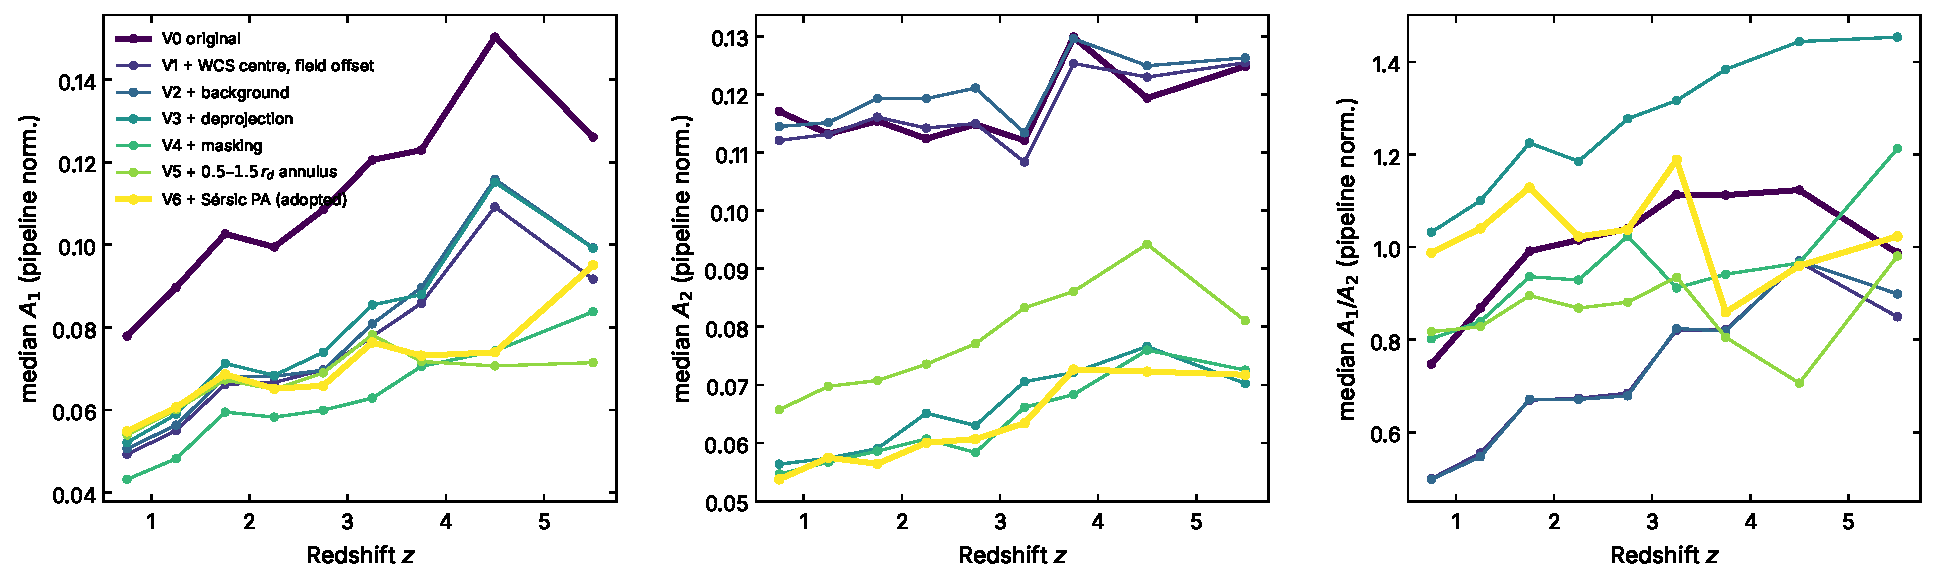
\includegraphics[width=0.95\textwidth]{Fig3_steps.pdf}
\caption{Median $A_1$ (left), $A_2$ (middle) and $A_1/A_2$ (right) of the
face-on disks as a function of redshift, as each correction is added to a
simple pipeline V0 (Table~\ref{tab:steps}; pipeline normalisation, no floor
or recovery correction). V1 uses the sub-pixel catalogue position, corrected
for the per-field astrometric offsets (Fig.~\ref{fig:astrometry}); V2
subtracts the sky background and keeps negative pixels; V3 deprojects the
azimuth, removing the $m=2$ power produced by the projection of a circular
disk; V4 masks neighbouring sources; V5 restricts the annulus to
$0.5$--$1.5\,r_d$; V6 uses the catalogue S\'ersic position angle and is the
adopted pipeline (thick yellow line; the $A_{\rm meas}$ of
Table~\ref{tab:chain}). Deprojection removes \numStepDeproj\ per cent of
$A_2$ at $z\sim0.75$, and the uncorrected pipeline V0 produces the spurious
rise of $A_1/A_2$ to $\approx\numStepVzeroR$.}
\label{fig:steps}
\end{figure*}

\subsubsection{Centring}\label{sec:centring}
The cutouts are aligned with the mosaic pixel grid, so a source sits at a random
sub-pixel position and the cutout centre can be off by up to half a pixel in
each coordinate. Since the $m=1$ mode is degenerate with a rigid shift of the
integration centre, this is the largest single source of spurious $A_1$ at small
apertures. To test the catalogue positions themselves, we took $\approx250$
compact, high-S/N point sources per filter and compared their centroids with the
catalogue positions (Fig.~\ref{fig:astrometry}).

\begin{figure}
\centering
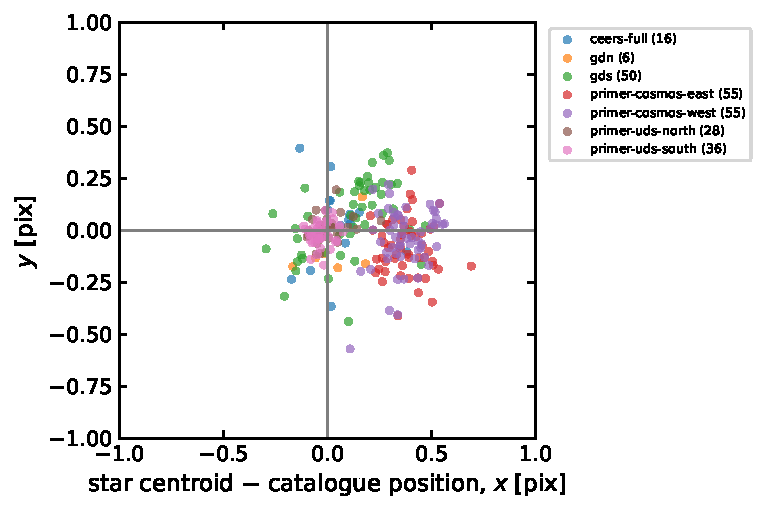
\includegraphics[width=0.95\columnwidth]{Fig4_astrometry.pdf}
\caption{Offset between the centroid of each point source in the F444W
cutouts and its catalogue position, coloured by field (number of stars in
parentheses). The stars in the two PRIMER-COSMOS mosaics share an offset of
$+0.37\,{\rm pix}$ in $x$ (identical in F150W, F200W, F277W, F356W and
F444W), while the other fields show offsets $\lesssim0.13\,{\rm pix}$. Such
a systematic, filter-independent offset points to an astrometric
calibration residual in the mosaic reduction rather than to a per-filter
PSF asymmetry, and acts on $A_1$ like a centring error. It is corrected
in step V1 (Table~\ref{tab:steps}).}
\label{fig:astrometry}
\end{figure}

The stars in both PRIMER-COSMOS mosaics are offset by $+0.37\,{\rm pix}$
($0.018\arcsec$) in $x$, by the same amount in F150W, F200W, F277W, F356W and
F444W, whereas the other fields show offsets $\lesssim0.13\,{\rm pix}$. After a
per-field correction the residual centring error is $0.10\,{\rm pix}$ per axis,
which corresponds to a floor $A_1^{\rm centring}\lesssim0.02$ at $r=5$~pix. Using
the sub-pixel position with these per-field offsets (step V1) lowers the median
$A_1$ by \numStepWcs\ per cent at $z<4$.

\subsubsection{Projection and neighbours}
Without deprojection, the projected ellipticity of $q=0.7$--$0.95$ disks
accounts for \numStepDeproj\ per cent of $A_2$ at $z\sim0.75$, as expected from
the geometric relation $A_2^{\rm proj}\simeq(1-q^2)/(1+q^2)$. Masking neighbours
inside the annulus lowers the median $A_1$ by \numStepMaskLo\ per cent on average
at $z<4$ and by \numStepMaskHi\ per cent at $z>4$.

\subsubsection{PSF}
At the $0.05\arcsec$ sampling of the cutouts, the stacked empirical PSFs have
FWHMs of $0.112$, $0.123$, $0.134$, $0.139$ and $0.156\arcsec$ in F150W, F200W,
F277W, F356W and F444W. At $z\sim4.5$ the median disk radius of the measured
galaxies is \numRdHiPix\,pix, compared with an F444W FWHM of \numFwhmPix\,pix
($r_d/{\rm FWHM}\approx\numRdFwhm$). The PSF therefore suppresses both modes
substantially, and $m=2$ more than $m=1$, since higher-order azimuthal structure
is smoothed more strongly at fixed radius.

\subsubsection{Noise}
Pixel noise in the cutouts is correlated, as expected for resampled (drizzled)
mosaics \citep{FruchterHook2002}. The nearest-neighbour autocorrelation in F444W
is $0.30$, the same in all seven mosaics, and the variance in an aperture is
$\approx6$ times the white-noise value. Unless this correlation is modelled, the
injection simulations underestimate the noise floor and overestimate the
recovered fraction, so we measure the autocorrelation on masked sky pixels in
each filter and use it in the simulations below.

\subsection{Injection--recovery calibration}\label{sec:injection}

Two biases remain once the pipeline is complete. Noise adds a positive bias
that no choice of aperture can remove and that has to be subtracted
statistically; the PSF suppresses the amplitudes, and this has to be divided out
with a model-based correction. For each redshift bin we draw 300 galaxies from
the observed sample, keeping their $r_d$, $n$, $q$ and aperture S/N. In bins with
fewer galaxies the draw is made with replacement (e.g.\ from the 77 galaxies at
$z\sim5.5$), and only the injected galaxies that pass the selection of
Sect.~\ref{sec:data} are used. For each one we build a S\'ersic disk with known azimuthal
perturbations, convolve it with the empirical PSF, add noise with the measured
autocorrelation, displace the centre by the residual centring error and run the
same pipeline (Fig.~\ref{fig:injection}).

\begin{figure*}
\centering
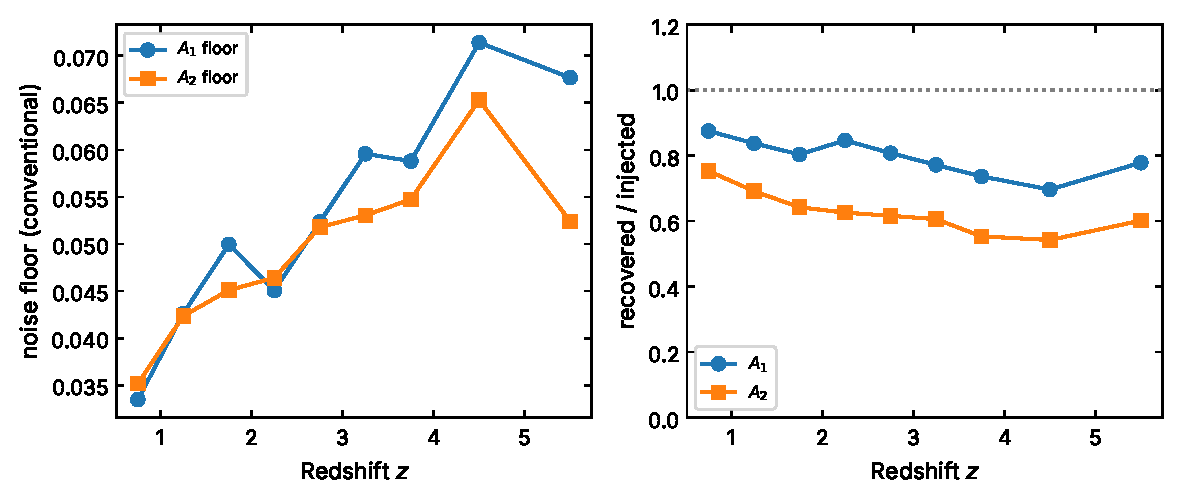
\includegraphics[width=0.95\textwidth]{Fig5_injection.pdf}
\caption{Injection--recovery calibration in F444W. \textit{Left:} noise
floor of $A_1$ and $A_2$ (conventional normalisation, twice the pipeline
values of Table~\ref{tab:chain}) for axisymmetric models with the observed
sizes, shapes and S/N, correlated noise and the empirical PSF. The floor
is almost identical for $m=1$ and $m=2$ at a given S/N but rises steeply
with redshift because the median S/N drops from $\approx500$ at
$z\sim0.75$ to $\approx100$ at $z\sim4.5$; it is the bias that noise
alone produces in the amplitude of a finite annulus. \textit{Right:}
fraction of the injected amplitude recovered after floor subtraction, for
injections at the observed amplitudes. The recovered fraction of $A_2$
drops faster than that of $A_1$ because the second harmonic has a smaller
angular scale, so the PSF suppresses it more severely as the galaxy
becomes smaller relative to the PSF at high redshift; the redshift
evolution of the recovered fraction mainly reflects the decrease of
$r_d/{\rm FWHM}$.}
\label{fig:injection}
\end{figure*}

Axisymmetric models give the noise floor: $A_1=\numFloorConvLow$ at
$z\sim0.75$, rising to $\numFloorConvHigh$ at $z\sim4.5$ in the conventional
normalisation (\numFloorPipeLow\ and \numFloorPipeHigh\ in the pipeline
normalisation of Table~\ref{tab:chain}) as the median S/N falls from
$\approx500$ to $\approx100$. We subtract it in quadrature. Models injected with
the final corrected amplitudes of Table~\ref{tab:main} give the recovered
fraction, \numRecOneRange\ for $A_1$ and \numRecTwoRange\ for $A_2$, which we
divide out. (The calibration is iterated; injecting the amplitudes from the
previous calibration changes no final value by more than $0.2\sigma$.) The
recovered fraction falls with redshift because the PSF suppresses $m=2$ more
strongly than $m=1$ as galaxies shrink relative to it. For the same reason the
measured $A_1/A_2$ of the simulated galaxies exceeds the injected value by a
factor \numBiasRange, which we also correct. Since the recovered fraction depends
on the injected amplitude (Table~\ref{tab:robust}), calibrating at amplitudes
much smaller than those observed would overestimate the correction.

\begin{table*}
\centering
\caption{Robustness of the growth of $A_1$ and $A_2$ and of the
corrected ratio. The last two columns are simple arithmetic means of
the corrected ratio in the bins below and above $z=3.5$; the
inverse-variance weighted means quoted in the abstract and in
Sect.~\ref{sec:ratio} are $\numRatioLo\pm\numRatioLoErr$ ($z<3.5$) and
$\numRatioHi\pm\numRatioHiErr$ ($z>3.5$) for the nominal row. $N_{z>4}$ is the
number of galaxies at $z>4$.}
\label{tab:robust}
\small
\begin{tabular}{lccccc}
\hline
{Test} & {$N_{z>4}$} & {$A_1$ growth} &
{$A_2$ growth} &
{$\langle A_1/A_2\rangle_{z<3.5}$} &
{$\langle A_1/A_2\rangle_{z>3.5}$}
\\
\hline
Nominal (Table~\ref{tab:main}) & 148 & 1.7 & 1.7 & 0.86 & 0.72\\
Self-consistent calibration, 2nd iteration & 148 & 1.7 & 1.7 & 0.86 & 0.72\\
Clumpy calibration (4 clumps, 20\% of flux) & -- & 1.7 & 1.6 & 0.89 & 0.69\\
Clumpy calibration (8 clumps, 30\% of flux) & -- & 1.7 & 1.6 & 0.88 & 0.77\\
Annulus 0.30--0.90\,$r_d$ & 46 & 1.2 & 1.5 & 1.07 & 0.71\\
Annulus 0.84--2.52\,$r_d$ & 225 & 2.6 & 1.7 & 0.65 & 0.71\\
Mass-matched to the pooled $M_\star$ distribution & 148 & 1.8 & 1.9 & 0.85 & 0.70\\
$9.0<\log M_\star<9.5$ & 37 & 2.0 & 1.9 & 0.81 & 0.66\\
$9.5<\log M_\star<10.0$ & 53 & 1.8 & 1.3 & 0.92 & 0.70\\
$10.0<\log M_\star<10.5$ & 20 & 0.9 & 1.4 & 0.84 & 0.48\\
$10.5<\log M_\star<11.5$ & 0 & -- & -- & 0.85 & 0.89\\
\hline
\end{tabular}
\end{table*}

All corrections are applied to the median amplitudes of each bin rather than
to individual galaxies:
\begin{eqnarray}
A_m^{\rm final} &=& 2\,\frac{\sqrt{(A_m^{\rm meas})^2-(A_m^{\rm floor})^2}}{f_{\rm rec}}, \nonumber\\
\left(\frac{A_1}{A_2}\right)_{\rm corr} &=& \frac{(A_1/A_2)_{\rm obs}}{b},
\label{eq:chain}
\end{eqnarray}
where $A_m^{\rm meas}$ is the median of the adopted pipeline (last row of
Table~\ref{tab:steps}), $A_m^{\rm floor}$ the median for axisymmetric models,
$f_{\rm rec}$ the median recovered fraction and $b$ the median ratio bias, all in
the pipeline normalisation; the factor 2 converts to the conventional
normalisation. The noise floor is a property of the distribution, and for a
single galaxy with $A_m<A_m^{\rm floor}$ the quadrature subtraction is
undefined. Within a bin, however, the floor and the recovered fraction are
constant, so the correction is a monotonic function of $A_m^{\rm meas}$. Applying
it galaxy by galaxy (with amplitudes below the floor set to zero) therefore
gives the same median as applying it to the median, and we have checked that
this reproduces Table~\ref{tab:main}. How well a single bin-level calibration
recovers the median of a population with a spread of sizes, S/N and amplitudes
is tested below and in Appendix~\ref{app:robust} (Table~\ref{tab:selection}). As an example, at $z\sim0.75$,
$A_1=2\sqrt{\numExAmeas^2-\numExAfloor^2}/\numExArec=\numExAresult$, and at
$z\sim4.5$, $A_2=2\sqrt{\numExBmeas^2-\numExBfloor^2}/\numExBrec=\numExBresult$;
Table~\ref{tab:main} gives \numExAtable\ and \numExBtable\ because it uses
unrounded inputs. Every term for every bin is listed in Table~\ref{tab:chain}
(Appendix~\ref{app:chain}). Since $f_{\rm rec}$ decreases with redshift, the
recovery correction contributes part of the measured growth (a factor
$1/\numExBrec=\numExBinv$ for $A_2$ at $z\sim4.5$). The amplitudes with only the
floor subtracted do not depend on it, although they still depend on the
noise-floor calibration (Sect.~\ref{sec:growth}).

The uncertainties of the final values combine the sampling error of the
observed galaxies with the calibration error. Both are obtained by bootstrapping
the observed galaxies of each bin together with the injected galaxies of the
noise-floor and recovery simulations. As a systematic test we repeat the
calibration with the injected amplitudes scaled by 0.5 and 1.5, and with
perturbations whose amplitude rises ($\propto r$) or falls ($\propto r^{-1}$)
with radius, and add the largest change of each final value in quadrature. All
uncertainties quoted for the final values (Table~\ref{tab:main}, figures and
text) are these totals,
$\sigma_{\rm tot}=(\sigma_{\rm stat+cal}^2+\sigma_{\rm syst}^2)^{1/2}$;
Table~\ref{tab:errors} lists the two parts separately. The ratio $A_1/A_2$ is
formed galaxy by galaxy before the median is taken, and it is bootstrapped
jointly with the two amplitudes, so the covariance of $A_1$ and $A_2$, which
share the same images, centring, deprojection and PSF, is contained in its
uncertainty. The growth factors compare disjoint sets of galaxies; their
uncertainties add the total errors of the two redshift ranges in quadrature,
i.e.\ the calibration systematics of different bins are treated as independent.
A systematic shared by all bins, such as an error in the PSF model or in the
injected amplitudes, largely cancels in a ratio of high- to low-redshift
amplitudes; the coherent PSF-model and injection-sampling variations of
Tables~\ref{tab:calsys} and \ref{tab:seeds}, applied to every bin at once, change
the growth factors by at most 0.06, which bounds this covariant contribution, so
the quadrature sum is conservative for the common-mode part.
The largest systematic term is that of $A_1$ at $z\sim4.5$ (0.060,
Table~\ref{tab:errors}), which dominates the uncertainty of its growth factor.

\begin{table*}
\centering
\caption{Error budget of Table~\ref{tab:main} (conventional
normalisation): joint bootstrap of the observed and injected galaxies
($\sigma_{\rm stat+cal}$), largest change among the four alternative
calibrations ($\sigma_{\rm syst}$), and their quadrature sum
($\sigma_{\rm tot}$), which is the uncertainty quoted in
Table~\ref{tab:main}.}
\label{tab:errors}
\small
\begin{tabular}{rccccccccc}
\hline
{} & \multicolumn{3}{c|}{$A_1$} & \multicolumn{3}{c|}{$A_2$} &
\multicolumn{3}{c}{$A_1/A_2$}\\
{$z$} & {$\sigma_{\rm stat+cal}$} &
{$\sigma_{\rm syst}$} & {$\sigma_{\rm tot}$} &
{$\sigma_{\rm stat+cal}$} & {$\sigma_{\rm syst}$} &
{$\sigma_{\rm tot}$} & {$\sigma_{\rm stat+cal}$} &
{$\sigma_{\rm syst}$} & {$\sigma_{\rm tot}$}
\\
\hline
0.75 & 0.004 & 0.004 & 0.006 & 0.005 & 0.002 & 0.006 & 0.037 & 0.032 & 0.049\\
1.25 & 0.006 & 0.006 & 0.009 & 0.007 & 0.004 & 0.008 & 0.048 & 0.084 & 0.097\\
1.75 & 0.006 & 0.013 & 0.015 & 0.007 & 0.005 & 0.009 & 0.056 & 0.053 & 0.078\\
2.25 & 0.008 & 0.006 & 0.009 & 0.011 & 0.008 & 0.014 & 0.058 & 0.046 & 0.074\\
2.75 & 0.011 & 0.005 & 0.012 & 0.014 & 0.011 & 0.018 & 0.075 & 0.057 & 0.095\\
3.25 & 0.012 & 0.025 & 0.028 & 0.014 & 0.004 & 0.015 & 0.086 & 0.132 & 0.157\\
3.75 & 0.010 & 0.027 & 0.029 & 0.026 & 0.017 & 0.031 & 0.095 & 0.050 & 0.108\\
4.50 & 0.024 & 0.060 & 0.065 & 0.035 & 0.044 & 0.056 & 0.094 & 0.060 & 0.111\\
5.50 & 0.037 & 0.024 & 0.044 & 0.042 & 0.009 & 0.043 & 0.100 & 0.065 & 0.119\\
\hline
\end{tabular}
\end{table*}

Because the injected galaxies are drawn from the observed sample of each bin,
their median disk radius and axis ratio agree with those of the measured
galaxies to within \numInjRdDev\ per cent and \numInjQDev, respectively. Each bin
is corrected at its median amplitude, so we also tested whether this recovers
the median of a population with a spread of amplitudes. To do so, we combined the
injections at 0.5, 1 and 1.5 times the observed amplitudes in different
proportions (\texttt{median\_recovery\_test.py}). For a uniform mixture the
median is recovered to within \numMedUni\ per cent. If most galaxies lie below
the calibration amplitude, the amplitudes are overestimated by \numMedLowAone\
($A_1$) and \numMedLowAtwo\ ($A_2$) per cent on average; if most lie above it,
they are underestimated by about \numMedHighAone\ per cent. The corrected
$A_1/A_2$ changes by at most \numMedRatio\ per cent. Smooth S\'ersic models
cannot capture clumpy, irregular light distributions, so these corrections remain
approximate.

We tested three further aspects of the calibration on the same injected
galaxies. All variants use identical models and noise fields, so that their
differences are not washed out by sampling noise (Table~\ref{tab:calsys}).

\textit{Deprojection parameters.} The simulations deproject each model with the
axis ratio and position angle used to build it. The observed galaxies, in
contrast, are deprojected with catalogue values that carry errors, and the DJA
catalogue gives no uncertainties for them. We therefore re-measured every
injected galaxy with perturbed $(q,{\rm PA})$ and re-derived the noise floor,
recovered fraction and ratio bias. Two kinds of perturbation were used: (a) the
noise-induced errors measured on the injected images themselves
($\sigma_q=0.004$--0.019 and $\sigma_{\rm PA}=1.5^\circ$--$6^\circ$ from
$z\sim0.75$ to $z>4$), and twice these errors; and (b) PA errors drawn from the
observed differences between the catalogue S\'ersic PA and the second-moment PA
of real galaxies in the same redshift bin and axis-ratio tercile (robust scatter
from $11^\circ$ at $z\sim0.75$ to $30^\circ$ at $z\sim5.5$), applied in full and
divided by $\sqrt2$. These differences depend only weakly on ellipticity: their
robust scatter is 1.5--2 times larger in the roundest than in the most elongated
quartile, whereas pure measurement noise would give $\approx3$. They must
therefore include structural differences between the annulus and the galaxy as a
whole. At the same time, $|\Delta{\rm PA}|$ correlates with $A_2$ measured with
the catalogue PA, and increasingly so with ellipticity (Spearman $\rho=0.02$ to
0.21), as expected if part of the difference is an error in the catalogue PA.
Without an independent, e.g.\ kinematic \citep{Wisnioski2015}, position angle
the two contributions cannot be separated, and we treat scenario (b) as a
conservative upper limit.

For scenario (a) the growth factors change by at most 0.05 ($A_1$) and 0.11
($A_2$). A centrally symmetric distortion of the coordinates cannot create odd
harmonics, so $A_1$ is affected only through the mask and the annulus. Scenario
(b) is more severe for $A_2$: PA errors as large as the empirical differences
add spurious $m=2$ power to the simulated galaxies, most strongly at high
redshift, where the differences are largest, and the growth factor of $A_2$ falls
from 1.76 to 1.74, 1.51 and 1.44 for the three variants of
Table~\ref{tab:calsys}, while that of $A_1$ rises from 1.65 to 1.70--1.78. If the
whole of the empirical PA difference were an error of the catalogue, $A_2$ would
thus grow by a factor of about 1.5 rather than 1.7. As a stress test we also
applied fixed Gaussian errors at every redshift,
$(\sigma_q,\sigma_{\rm PA})=(0.02,2^\circ)$, $(0.05,5^\circ)$ and
$(0.10,10^\circ)$. The first two change the growth factors by $\leq0.10$. The
largest, whose $\sigma_q$ is 5--25 times the measured noise-induced error, raises
the growth factor of $A_2$ to 2.03, because errors of this kind add spurious
$m=2$ power of similar absolute size at all redshifts, which is a larger fraction
of the small $A_2$ at low redshift.

The corrected ratio $A_1/A_2$ is sensitive in the same way. PA errors of the
empirical size lower the ratio bias and raise the corrected ratio from 0.88 to
0.94--0.99 at $z<3.5$ and from 0.71 to 0.76--0.83 at $z>3.5$. We therefore give
the corrected ratio a one-sided systematic uncertainty of $+0.11$ ($z<3.5$) and
$+0.12$ ($z>3.5$). In every case it stays below unity on average, and lower at
$z>3.5$ than at $z<3.5$; only the largest stress test brings its mean at $z<3.5$
to 1.01.

\textit{PSF.} Repeating the calibration with 100 PSFs stacked from bootstrap
resamples of the 246 stars changes the corrected amplitudes by $\leq0.002$
(r.m.s.) in every bin, and the growth factors by 0.003 ($A_1$) and 0.004
($A_2$). This measures the uncertainty due to the finite set of stars, not systematic
errors in the PSF model itself. PSFs stacked separately in the CEERS, GOODS-S and PRIMER
fields, an azimuthally averaged PSF (no ellipticity or diffraction structure) and
a radial rescaling of the PSF by $\pm5$ per cent change the growth factors by at
most 0.01 ($A_1$) and 0.05 ($A_2$).

\textit{Sampling of the injections.} Repeating the calibration with 26
independent draws of the injected galaxies gives a scatter of 0.017--0.030 in the
recovered fractions and 0.002--0.010 in the corrected amplitudes
(Table~\ref{tab:seeds}). We compare the draws with Table~\ref{tab:main} in two
separate ways. (1) Bin by bin: comparing each draw with the mean and scatter of
the others gives an empirical reference distribution for the $\chi^2$ of the nine
bins. The values of Table~\ref{tab:main} are exceeded in 8--46 per cent of the
draws (empirical tail fractions, not classical $p$-values) for the recovered
fractions and corrected amplitudes of both modes, so the per-bin values are
consistent with the sampling of the injections, although the recovered fraction
of $A_1$ is in the tail (8 per cent). (2) Growth factors: over the draws these
are $1.70\pm0.04$ ($A_1$) and $1.65\pm0.06$ ($A_2$). The values of
Table~\ref{tab:main} (1.74 and 1.71) lie at the 81st and 85th percentiles of
these distributions, i.e.\ the adopted draw is slightly high for both modes, by
less than $1\sigma$ of the sampling scatter and by 0.1--0.2 of the total
uncertainties ($\pm0.3$). This sampling noise is already part of the joint
bootstrap of observed and injected galaxies, since the bootstrap uncertainties of
the recovered fractions in Table~\ref{tab:main} (0.018--0.036) match the scatter
between the draws; it is therefore not added again in Table~\ref{tab:errors}.

\begin{table*}
\centering
\caption{Sensitivity of the growth factors and of the mean corrected
ratio to the deprojection parameters and to the PSF model
(Sect.~\ref{sec:injection}). Each row repeats the injection--recovery
calibration (300 galaxies per bin; identical models and noise fields for all
rows) and re-derives Table~\ref{tab:main} from the observed medians. The
reference row uses the adopted inputs with this set of injected galaxies;
its differences from Table~\ref{tab:main} are due to the sampling of the
injections (Table~\ref{tab:seeds}). The last two columns are simple
arithmetic means, as in Table~\ref{tab:robust}.}
\label{tab:calsys}
\small
\begin{tabular}{lcccc}
\hline
{Calibration} & {$A_1$ growth} & {$A_2$ growth} &
{$\langle A_1/A_2\rangle_{z<3.5}$} & {$\langle A_1/A_2\rangle_{z>3.5}$}
\\
\hline
Reference (adopted inputs, true $q$ and PA)       & 1.65 & 1.76 & 0.88 & 0.71\\
\multicolumn{5}{l}{\textit{Deprojection: noise-induced errors measured on the injected images}}\\
Noise-induced errors                              & 1.70 & 1.74 & 0.87 & 0.75\\
Twice the noise-induced errors                    & 1.69 & 1.65 & 0.89 & 0.75\\
Noise-induced error in $q$ only                   & 1.67 & 1.65 & 0.87 & 0.72\\
Noise-induced error in PA only                    & 1.68 & 1.71 & 0.88 & 0.73\\
\multicolumn{5}{l}{\textit{Conservative upper limit: empirical PA differences}}\\
Empirical PA differences$/\sqrt2$                 & 1.70 & 1.74 & 0.94 & 0.76\\
Empirical PA differences                          & 1.75 & 1.51 & 0.98 & 0.81\\
Empirical PA differences, twice the $q$ error     & 1.78 & 1.44 & 0.99 & 0.83\\
\multicolumn{5}{l}{\textit{Stress test: fixed errors at every redshift}}\\
$\sigma_q=0.02$, $\sigma_{\rm PA}=2^\circ$         & 1.68 & 1.69 & 0.89 & 0.74\\
$\sigma_q=0.05$, $\sigma_{\rm PA}=5^\circ$         & 1.70 & 1.66 & 0.91 & 0.73\\
$\sigma_q=0.10$, $\sigma_{\rm PA}=10^\circ$        & 1.72 & 2.03 & 1.01 & 0.80\\
\multicolumn{5}{l}{\textit{PSF model}}\\
Bootstrap of the stars (100 PSFs; mean $\pm$ s.d.) & $1.648\pm0.003$ & $1.754\pm0.004$ & $0.878\pm0.001$ & $0.708\pm0.001$\\
CEERS stars only                                  & 1.65 & 1.78 & 0.88 & 0.71\\
GOODS-S stars only                                & 1.66 & 1.77 & 0.88 & 0.71\\
PRIMER stars only                                 & 1.64 & 1.74 & 0.88 & 0.72\\
Width $-5$ per cent                               & 1.64 & 1.74 & 0.88 & 0.71\\
Width $+5$ per cent                               & 1.66 & 1.81 & 0.87 & 0.69\\
Azimuthal average                                 & 1.65 & 1.78 & 0.88 & 0.71\\
\hline
\end{tabular}
\par\vspace{2pt}\begin{minipage}{\textwidth}\footnotesize\textit{Note.} Noise-induced errors: $q$ and PA from flux-weighted second
moments of each noisy injected image minus those of the noiseless convolved
image. Empirical PA differences: catalogue S\'ersic PA minus second-moment PA
of the observed galaxies, drawn in the same redshift bin and axis-ratio
tercile of the face-on sample before the S/N cut (an upper limit on the
catalogue PA error).\end{minipage}
\end{table*}

\begin{table*}
\centering
\caption{Sampling of the injected galaxies: mean $\pm$ standard
deviation over 26 independent draws of the injection calibration, with the
values of Table~\ref{tab:main} in parentheses. Against an empirical
leave-one-out reference distribution of $\chi^2$ over the nine bins, the
$\chi^2$ of the values of Table~\ref{tab:main} is exceeded in 8
($f_{\rm rec}$ of $A_1$), 35 ($f_{\rm rec}$ of $A_2$), 12 ($A_1$) and 46
($A_2$) per cent of the draws (empirical tail fractions). The growth factors of
Table~\ref{tab:main} lie at the 81st ($A_1$) and 85th ($A_2$) percentiles of the
draws.}
\label{tab:seeds}
\small
\begin{tabular}{rcccccccc}
\hline
{$z$} & \multicolumn{2}{c}{$f_{\rm rec}(A_1)$} & \multicolumn{2}{c}{$f_{\rm rec}(A_2)$} &
\multicolumn{2}{c}{$A_1$} & \multicolumn{2}{c}{$A_2$}
\\
\hline
0.75 & $0.851\pm0.019$ & (0.875) & $0.724\pm0.019$ & (0.753) & $0.122\pm0.002$ & (0.119) & $0.140\pm0.004$ & (0.135)\\
1.25 & $0.820\pm0.017$ & (0.838) & $0.669\pm0.022$ & (0.691) & $0.139\pm0.002$ & (0.136) & $0.159\pm0.005$ & (0.154)\\
1.75 & $0.806\pm0.019$ & (0.804) & $0.629\pm0.025$ & (0.642) & $0.160\pm0.004$ & (0.159) & $0.163\pm0.006$ & (0.161)\\
2.25 & $0.795\pm0.019$ & (0.847) & $0.623\pm0.019$ & (0.626) & $0.153\pm0.004$ & (0.144) & $0.176\pm0.005$ & (0.177)\\
2.75 & $0.771\pm0.030$ & (0.808) & $0.595\pm0.028$ & (0.616) & $0.157\pm0.006$ & (0.150) & $0.183\pm0.009$ & (0.178)\\
3.25 & $0.776\pm0.020$ & (0.772) & $0.601\pm0.023$ & (0.606) & $0.184\pm0.005$ & (0.182) & $0.191\pm0.008$ & (0.190)\\
3.75 & $0.774\pm0.021$ & (0.737) & $0.596\pm0.018$ & (0.553) & $0.176\pm0.005$ & (0.182) & $0.227\pm0.007$ & (0.243)\\
4.50 & $0.743\pm0.028$ & (0.696) & $0.551\pm0.024$ & (0.542) & $0.179\pm0.006$ & (0.186) & $0.235\pm0.010$ & (0.238)\\
5.50 & $0.769\pm0.022$ & (0.778) & $0.575\pm0.024$ & (0.601) & $0.234\pm0.007$ & (0.228) & $0.227\pm0.009$ & (0.222)\\
\hline
growth & & & & & $1.70\pm0.04$ & (1.74) & $1.65\pm0.06$ & (1.71)\\
\hline
\end{tabular}
\end{table*}



\subsection{Closure across field depth and the S/N limit}\label{sec:closure}

The seven fields differ in depth: at $z>4$ the median aperture S/N of the
face-on galaxies is 118 in CEERS and the two GOODS fields, 43 in PRIMER-COSMOS
and 26 in PRIMER-UDS. Since the selection in mass and catalogue S/N is the same
everywhere, galaxies of a given redshift and stellar mass are observed at
different S/N in different fields, and a correct noise calibration must return
the same amplitude for them. This is a test of the injection--recovery
calibration that does not rely on the simulations themselves.

Without an S/N limit the test fails (left half of Table~\ref{tab:closure}). At
$z\sim0.75$ the corrected amplitudes of the seven fields agree ($\chi^2=2.5$ for
$A_1$ and 11.2 for $A_2$, 6 degrees of freedom), but at $z>4$ they do not
($\chi^2=28$ and 39), and the growth factors follow the depth of the field: 1.2
and 1.4 in the deep fields, 2.0 and 2.4 in PRIMER-COSMOS, 2.8 and 4.2 in
PRIMER-UDS. Three observations show that the difference is one of S/N rather
than of field. (i) Within a common S/N tercile of the $z>4$ galaxies the raw
medians of the three groups agree within their errors (e.g.\ $A_1=0.15$--0.18 in
the lowest tercile, 0.10--0.11 in the middle one and 0.05--0.08 in the highest,
pipeline normalisation). (ii) The raw amplitudes anticorrelate with S/N at
$z>4$ (Spearman $\rho\approx-0.5$ for both modes), far more than at $z<2$
($\rho\approx-0.1$). (iii) The discrepancy survives a correction made galaxy by
galaxy: with a noise floor that depends on the S/N of each galaxy
($\log A^{\rm floor}=a+b\log{\rm S/N}$, fitted in each redshift bin to the
axisymmetric injections) and the recovered fraction of its S/N tercile, galaxies
with $9.0<\log\Mstar<9.5$ at $z>4$ have $A_1=0.15\pm0.05$, $0.25\pm0.03$ and
$0.33\pm0.02$ in the deep fields, PRIMER-COSMOS and PRIMER-UDS (median S/N of 65,
31 and 13), and $A_2=0.19\pm0.08$, $0.36\pm0.10$ and $0.69\pm0.12$. The median
masses of the three groups agree to 0.1\,dex, so the difference, $3.4\sigma$
between the deepest and shallowest group in each mode, is not a mass effect. At
$z\sim0.75$, at $z\sim3.75$ and for $\log\Mstar>10$ at $z>4$, where the S/N is
higher, the groups agree.

At low S/N the simulations therefore underestimate the bias of the amplitudes.
Two further tests, both in the supplementary material, show that this excess
belongs to the low-S/N galaxies themselves rather than to a systematic of the
measurement. At fixed stellar mass the per-galaxy corrected amplitude scales as
$\propto({\rm S/N})^{-0.33}$ for both modes at $z>3.5$
(\texttt{diagnose\_excess.py}); the slope is unchanged when the masked-pixel
fraction and the bright-neighbour density are added, and once the S/N and mass
trends are removed the residual field-to-field differences are $\leq0.06$\,dex,
so the excess tracks S/N and not crowding or the field. We also injected the same
models onto blank patches of the real sky of each field
(\texttt{real\_sky\_injection.py}, eight realisations), which carry the faint
undetected sources, background structure and pixel correlation that smooth models
with synthetic noise omit; compared at the same S/N the real-sky noise floor is
$1.1$--$1.3$ times the synthetic one for $A_1$ and consistent with it for $A_2$,
with no trend in S/N; applied to the full sample (without the S/N limit, the
relevant comparison for this test) the real-sky calibration leaves the growth
factors almost unchanged ($1.94\pm0.20$ and $2.01\pm0.09$, against the synthetic
1.98 and 2.32, and distinct from the adopted S/N$\,\geq40$ values of
Table~\ref{tab:main}), so an underestimated noise floor is not the cause. We conclude that the excess is intrinsic to the faint, poorly resolved
low-S/N galaxies. In addition, 9 and 16 per cent of the galaxies at
$z\sim4.5$ and $z\sim5.5$ have an aperture S/N below the lowest value in the
injections (10.4). Rather than model the excess, we restrict the sample to the
S/N range in which the test is passed. We fixed the criterion beforehand: a
threshold is accepted if, at $z\sim3.75$ and at $z>4$ and for both modes, every
pair of the three field groups agrees within $2\sigma$ and the $\chi^2$ of the
three about their weighted mean is below 5.99 (95 per cent for 2 degrees of
freedom), and if all higher thresholds are accepted as well. With the
galaxy-by-galaxy correction above, the largest pair difference is $2.5\sigma$
for S/N$\,\geq20$, $2.2\sigma$ for S/N$\,\geq30$, and $1.2$, $1.1$, $1.3$ and
$1.5\sigma$ for S/N$\,\geq40$, 50, 75 and 100. We adopt S/N$\,\geq40$. This is
not an effect of the growing errors alone: the median $A_2$ of PRIMER-UDS at
$z>4$ falls from 0.59 without a limit to 0.45 (S/N$\,\geq30$) and 0.29
(S/N$\,\geq40$), against 0.20--0.22 in the deep fields throughout. The growth
factors of the whole sample in the same test are 1.83 and 2.38 without a limit
and 1.51 and 1.56, 1.49 and 1.55, 1.50 and 1.42, 1.30 and 1.62 for the four
accepted thresholds, with uncertainties of 0.2--0.3, so the result does not
depend on the exact choice.

All calibrations of Sect.~\ref{sec:injection} were then repeated for the
S/N-limited sample, with injections drawn from it. With the new bin-level
calibration the seven fields are consistent in their growth factors
($\chi^2=7.4$ for $A_1$ and 10.8 for $A_2$, 6 degrees of freedom; right half of
Table~\ref{tab:closure}). Two residuals remain visible: PRIMER-UDS still has the
largest growth of $A_2$ (mainly its northern mosaic, $4.2\pm1.1$ from 19 galaxies
at $z>4$), and $A_1$ does not grow in GOODS-N ($1.05\pm0.25$, 35 galaxies).
Without the two UDS mosaics the growth factors are $1.48\pm0.20$ ($A_1$) and
$1.57\pm0.18$ ($A_2$). The growth factors of about 2.0 and 2.3 that the full
sample gives (Table~\ref{tab:closure}) are thus inflated by low-S/N galaxies in
the shallow fields, and all results below refer to the S/N-limited sample.

\begin{table*}
\centering
\caption{Closure test across field depth: growth factors of the corrected
amplitudes between $z\sim0.75$ and $z>4$ for groups of fields, without an S/N
limit and for aperture S/N$\,\geq40$, each with the bin-level calibration of its
own sample (which is approximate for subsets). $N_{z>4}$ is the number of
galaxies at $z>4$ and $\langle{\rm S/N}\rangle$ their median aperture S/N.
Uncertainties are bootstrap standard deviations over the observed galaxies. The
last row gives the $\chi^2$ of the logarithmic growth factors of the seven
individual mosaics about their weighted mean (6 degrees of freedom).}
\label{tab:closure}
\small
\begin{tabular}{lccccccc}
\hline
 & \multicolumn{4}{c}{no S/N limit} & \multicolumn{3}{c}{S/N$\,\geq40$}\\
Fields & $N_{z>4}$ & $\langle{\rm S/N}\rangle$ & $A_1$ growth & $A_2$ growth & $N_{z>4}$ & $A_1$ growth & $A_2$ growth\\
\hline
CEERS, GOODS-N, GOODS-S & 89 & 118 & $1.24\pm0.25$ & $1.41\pm0.25$ & 74 & $1.39\pm0.26$ & $1.65\pm0.23$\\
PRIMER-COSMOS (east, west) & 73 & 43 & $2.04\pm0.28$ & $2.40\pm0.37$ & 39 & $1.74\pm0.35$ & $1.72\pm0.31$\\
PRIMER-UDS (north, south) & 98 & 26 & $2.83\pm0.28$ & $4.23\pm0.56$ & 35 & $1.92\pm0.43$ & $2.85\pm0.82$\\
All fields & 260 & -- & $1.98\pm0.14$ & $2.32\pm0.32$ & 148 & $1.74\pm0.19$ & $1.71\pm0.20$\\
\hline
$\chi^2$ of the seven mosaics & & & 21.9 & 32.1 & & 7.4 & 10.8\\
\hline
\end{tabular}
\end{table*}

%% -----------------------------------------------------------------------
\section{Results}\label{sec:results}

\subsection{Growth of $A_1$ and $A_2$}\label{sec:growth}

Table~\ref{tab:main} and Fig.~\ref{fig:amplitudes}, which are generated from
the same output table, give the corrected amplitudes of the face-on disks. Both
modes grow with redshift. $A_1$ rises from $\numAOneLow$ at $z\sim0.75$ to
$\numAOneHigh$ at $z>4$, a factor of $\numAOneGrowth\pm0.3$, and $A_2$ from
$\numATwoLow$ to $\numATwoHigh$, a factor of $\numATwoGrowth\pm0.3$; here the
$z>4$ values are the mean of the $z\sim4.5$ and $z\sim5.5$ bins, and the
uncertainties propagate the total errors of Table~\ref{tab:main}. These
end-point ratios rest on the 148 galaxies at $z>4$. A fit of
$\log A=a+b\log(1+z)$ to all nine bins uses the whole sample and gives
$b=0.38\pm0.08$ for $A_1$ and $0.43\pm0.07$ for $A_2$ ($\chi^2=3.8$ and 2.6 for
7 degrees of freedom, with the total errors of the bins treated as independent),
which corresponds to factors of 1.6 and 1.7 between $z=0.75$ and $z=5$. The two
slopes agree. The growth factors quoted in this paper for the S/N-limited sample
come from several calibrations, and their spread is part of the uncertainty: the
adopted bin-level calibration gives 1.74 and 1.71 (Table~\ref{tab:main}), the
mean over 26 independent draws of the injected galaxies 1.70 and 1.65
(Table~\ref{tab:seeds}), a second run with 600 injections per bin 1.62 and 1.70,
or 1.59 and 1.64 when it is stratified in S/N (Table~\ref{tab:selection}), and
the galaxy-by-galaxy noise floor of Sect.~\ref{sec:closure}, which is fitted to
the injections of the sample without an S/N limit, 1.51 and 1.56. All lie within
the quoted uncertainty of $\pm0.3$, and none separates the two modes. With only the noise floor subtracted, the growth factors are
$\numAOneGrowthFloor\pm0.16$ and $\numATwoGrowthFloor\pm0.15$ and the slopes
$0.27\pm0.04$ and $0.16\pm0.05$. These do not depend on the model-based recovery
correction, though they do depend on the noise-floor calibration. Because the PSF
can only suppress the amplitudes, and the recovered fraction does not increase
with redshift in the simulations (Table~\ref{tab:chain}), they are lower limits
on the growth. For $A_2$ a large part of the growth therefore comes from the
recovery correction, which rises from $1/0.75$ at $z\sim0.75$ to $1/0.54$ at
$z\sim4.5$: the growth of $A_2$ without it is significant at only the
$2$--$3\sigma$ level.

\begin{figure*}
\centering
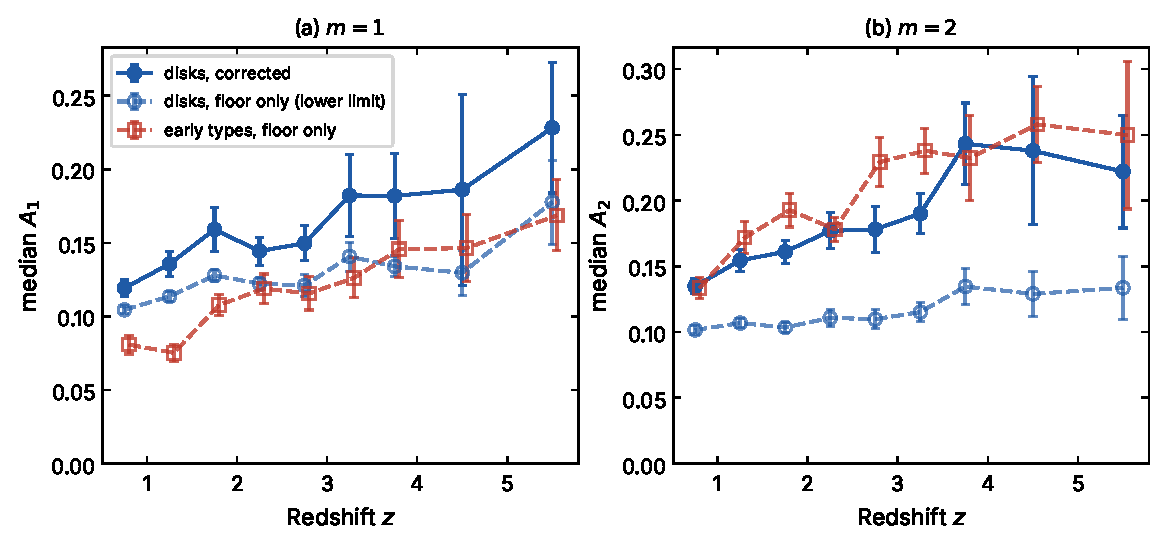
\includegraphics[width=0.95\textwidth]{Fig1_amplitudes.pdf}
\caption{Median $A_1$ (left) and $A_2$ (right) as a function of redshift.
Filled circles: face-on disks corrected for the noise floor and the
PSF/noise recovery fraction (Eq.~\ref{eq:chain}); open circles: noise
floor subtracted only (lower limits, independent of any model-based
recovery correction); open squares: early-type galaxies ($n>3$), noise
floor subtracted only. Both $A_1$ and $A_2$ grow by a factor of about 1.7
between $z\sim0.75$ and $z>4$; the two modes grow by comparable factors,
in contrast to a bar-driven increase (which would raise $A_2$ at nearly
constant $A_1$) or a lopsided-mode increase (which would raise $A_1$ at
nearly constant $A_2$). The lower-limit curves also rise, by factors of
\numAOneGrowthFloor\ and \numATwoGrowthFloor, so the growth is not produced by the
model-based recovery correction alone, although for $A_2$ that correction
supplies most of it.
Early-type galaxies show a similar growth of both modes.}
\label{fig:amplitudes}
\end{figure*}

\subsection{Rest-frame wavelength}\label{sec:restframe}

F444W samples $2.5\,\mu$m in the rest frame at $z=0.75$ but $0.8\,\mu$m at
$z=4.5$. A trend measured in one filter could therefore reflect the changing
rest-frame tracer rather than an intrinsic change in asymmetry: shorter
wavelengths probe younger stars and clumpier star formation, and local galaxies
show larger $A_m$ at shorter wavelengths \citep{Buta2015}. For the same galaxies,
the median ratio of the amplitudes measured in F277W and F444W is
\numFRoneRange\ for $A_1$ and \numFRtwoRange\ for $A_2$ across the nine redshift
bins, while the rest wavelengths differ by a factor of 1.6. F277W and F444W have
similar PSFs and S/N, so this comparison needs no model correction. $A_1$ is
thus nearly independent of wavelength, whereas $A_2$ is larger at shorter
wavelengths, as expected if the $m=2$ mode traces younger, clumpier,
dust-affected star formation.

Scaled to the factor of 3.2 in rest wavelength that F444W spans between
$z=0.75$ and $z=4.5$, the change of wavelength alone could raise $A_1$ by
$\lesssim\numFRexpectOne$ and $A_2$ by $\lesssim\numFRexpectTwo$ per cent,
compared with observed factors of \numAOneGrowth\ and \numATwoGrowth. Part of
the growth of $A_2$ in F444W may therefore be a change of tracer, and the
decisive test is a comparison at fixed rest wavelength. When we measure each
galaxy in the filter closest to a fixed rest wavelength and correct each filter
with its own simulations, the growth persists (Table~\ref{tab:restframe},
Fig.~\ref{fig:restframe}). Wavelength-dependent effects alone therefore cannot
explain the evolution, although this test does not by itself rule out other
contributions, such as residual resolution effects or changes in sample
composition with redshift. The F150W amplitudes of high-redshift galaxies are
systematically larger, but they probe the rest-frame ultraviolet at much lower
S/N, and we do not use them above $z\sim1.75$.

\begin{table*}
\centering
\caption{Corrected amplitudes at fixed rest-frame wavelength,
compared with F444W alone. Each galaxy is measured in the filter (F150W,
F277W or F444W) whose pivot wavelength divided by $(1+z)$ is closest to
the target, within 0.12\,dex. Each filter is corrected with its own
injection simulations, using the same centring scheme and matched
scenario as Table~\ref{tab:main}. $N$ is the number of galaxies, with
the filters contributing at $z\sim4.5$ being F444W except for three galaxies in
F277W in the $0.7\,\mu$m row. Uncertainties are bootstrap errors on the medians,
with the growth-factor error propagated from the two bins.}
\label{tab:restframe}
\small
\begin{tabular}{lcccccccc}
\hline
{} & \multicolumn{2}{c}{$N$} & \multicolumn{3}{c}{$A_1$} &
\multicolumn{3}{c}{$A_2$}\\
{} & {$z\sim0.75$} & {$z\sim4.5$} &
{$z\sim0.75$} & {$z\sim4.5$} & {growth} &
{$z\sim0.75$} & {$z\sim4.5$} & {growth}
\\
\hline
F444W only & 1311 & 97 & $0.119\pm0.003$ & $0.186\pm0.022$ & $1.6\pm0.2$ & $0.135\pm0.004$ & $0.238\pm0.032$ & $1.8\pm0.2$\\
$\lambda_{\rm rest}=0.7\,\mu$m & 1121 & 97 & $0.113\pm0.003$ & $0.185\pm0.022$ & $1.6\pm0.2$ & $0.146\pm0.005$ & $0.238\pm0.033$ & $1.6\pm0.2$\\
$\lambda_{\rm rest}=1.0\,\mu$m & 1204 & 90 & $0.109\pm0.002$ & $0.183\pm0.022$ & $1.7\pm0.2$ & $0.145\pm0.005$ & $0.241\pm0.035$ & $1.7\pm0.2$\\
\hline
\end{tabular}
\end{table*}


\begin{figure*}
\centering
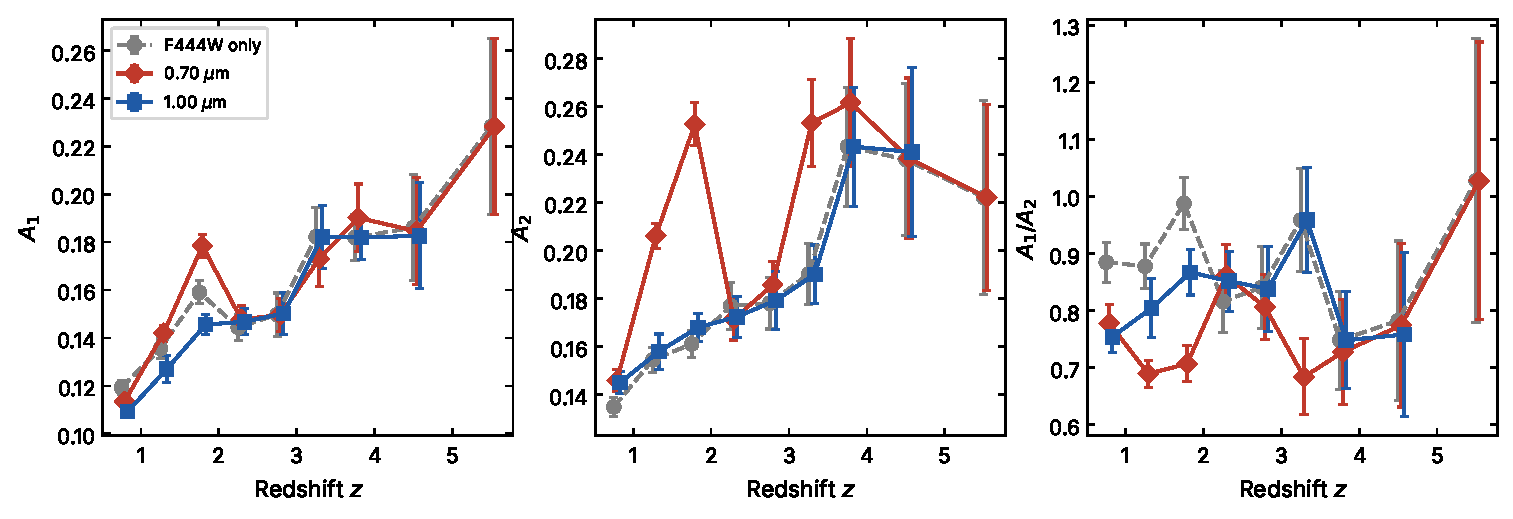
\includegraphics[width=0.95\textwidth]{Fig6_restframe.pdf}
\caption{$A_1$ (left), $A_2$ (middle) and $A_1/A_2$ (right) at fixed
rest-frame wavelength (0.7 and $1.0\,\mu$m) compared with F444W alone,
each filter corrected with its own simulations. For each galaxy the
filter is chosen whose pivot wavelength divided by $(1+z)$ is closest to
the target rest wavelength, within 0.12\,dex (Table~\ref{tab:restframe}).
The growth of $A_1$ and $A_2$ at fixed rest wavelength is close to that
in F444W alone and the ratio stays below unity throughout, so the
change of rest-frame tracer alone cannot explain the evolution. At
$1.0\,\mu$m, F150W dominates at $z\sim0.75$ and F444W at $z\sim4.5$, each
corrected with its own simulations.}
\label{fig:restframe}
\end{figure*}

\subsection{The ratio $A_1/A_2$}\label{sec:ratio}

The median observed per-galaxy ratio is $\numRobsLow$ at $z\sim0.75$ and
\numRobsHighRange\ at $z>1.5$. According to the simulations the PSF raises it by
a factor \numBiasRange: at a given $r_d/{\rm FWHM}$ the PSF suppresses $A_2$ more
than $A_1$, which pushes the ratio artificially upwards at high redshift. After
correction (Fig.~\ref{fig:ratio}) the ratio is $\numRcorrLow\pm\numRcorrLowErr$
at $z\sim0.75$, and its weighted mean over all bins is
$\numRatioMean\pm\numRatioMeanErr$, with $\chi^2=\numRatioChi$ for
$\numRatioDof$ degrees of freedom about this constant. The bins at $z>3.5$ lie
lower: their inverse-variance weighted mean is $\numRatioHi\pm\numRatioHiErr$,
against $\numRatioLo\pm\numRatioLoErr$ at $z<3.5$ (the simple arithmetic means in
Table~\ref{tab:robust} are 0.86 and 0.72), and a linear fit gives
${\rm d}(A_1/A_2)/{\rm d}\log(1+z)=\numRatioSlope\pm\numRatioSlopeErr$. The
difference between the two ranges is $0.13\pm0.07$, so the ratio is consistent
with a constant and at most declines mildly, as the equal slopes of the two
amplitudes (Sect.~\ref{sec:growth}) also indicate.
Catalogue position-angle errors of the size suggested by the data would raise
these values by up to 0.11 ($z<3.5$) and 0.12 ($z>3.5$;
Sect.~\ref{sec:injection}, Table~\ref{tab:calsys}). The absolute value of the
ratio is uncertain at this level, but in none of these calibrations does it rise
with redshift. At fixed rest-frame wavelength the ratio of the corrected
median amplitudes (without the ratio-bias correction) is \numRFratioRange\ at
$z\geq1.25$. We therefore find no evidence that lopsidedness comes to dominate
over bisymmetric structure at high redshift. The redshift trend of the ratio
does, however, depend on the radius of the annulus. In annuli 0.6 and 1.68 times
smaller and larger than ours its mean is $\numAnnSmallR$ and $\numAnnLargeR$; in
the smaller annulus it falls from 1.07 at $z<3.5$ to 0.71 at $z>3.5$, and in the
larger one it does not fall (0.65 and 0.71; Table~\ref{tab:robust}), so we do not
attach physical meaning to its mild decrease at $z>3.5$.

\begin{figure}
\centering
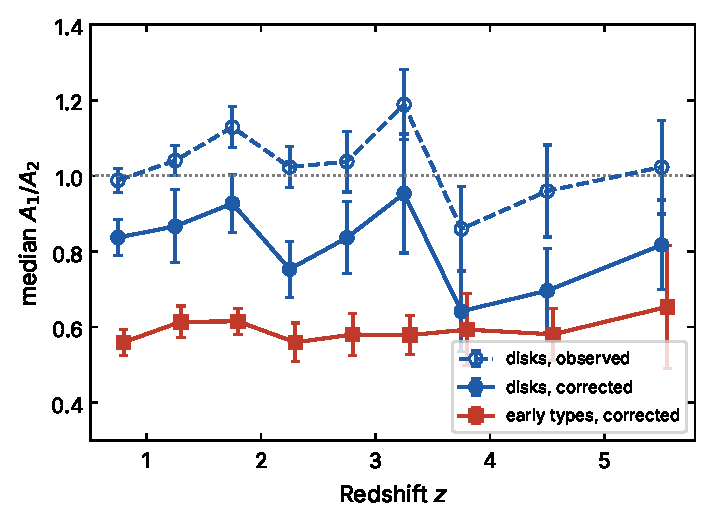
\includegraphics[width=0.95\columnwidth]{Fig2_ratio.pdf}
\caption{Median $A_1/A_2$ of face-on disks, observed (open) and
corrected for the PSF-induced ratio bias (filled), and of early-type
galaxies (corrected). The downward correction between the open and
filled curves is a direct consequence of the PSF suppressing $m=2$
more than $m=1$, as predicted by the injection simulations
(Fig.~\ref{fig:injection}). The corrected ratio of the disks stays
below unity at all redshifts within its uncertainties: $A_1$ does not come to
dominate over $A_2$. Errors in the catalogue position angles of the size suggested by the
data would raise the corrected ratio by up to 0.11 ($z<3.5$) and 0.12
($z>3.5$; Sect.~\ref{sec:injection}), which is not shown. Early-type galaxies have a lower corrected ratio
($\approx\numETratioR$; their ratio correction is approximate).}
\label{fig:ratio}
\end{figure}

\subsection{Star formation}\label{sec:sfr}

Star-formation rates and stellar masses come from the same DJA catalogue, at
the same row as the morphological parameters (the masses agree to
$2\times10^{-4}$\,dex). We classify galaxies relative to the main sequence of
\citet{Speagle2014} as star-forming ($\Delta_{\rm MS}>-0.3$) or quiescent
($\Delta_{\rm MS}<-1$). Quiescent disks are few (7 per cent of the sample) and,
at a given redshift, differ from star-forming ones in median aperture S/N by
factors of up to four in either direction. Restricting both classes to S/N$>100$,
which keeps the noise floor small and similar for the two, we find $A_1^{\rm SF}/A_1^{\rm Q}=\numSFQ\pm\numSFQerr$ at
$z\lesssim3$ (Fig.~\ref{fig:sfr}); at $z>3$ there are too few high-S/N quiescent
disks for this test. If internal lopsided modes of cold, rotation-supported
disks \citep{Jog1997,Saha2007} were preferentially excited in star-forming disks
with ongoing gas accretion, they would enhance $A_1$ in the star-forming class.
We see no such enhancement at $z\lesssim3$ in the high-S/N regime, although the
test is limited by the small number of high-S/N quiescent disks and by the
main-sequence classification.

\begin{figure*}
\centering
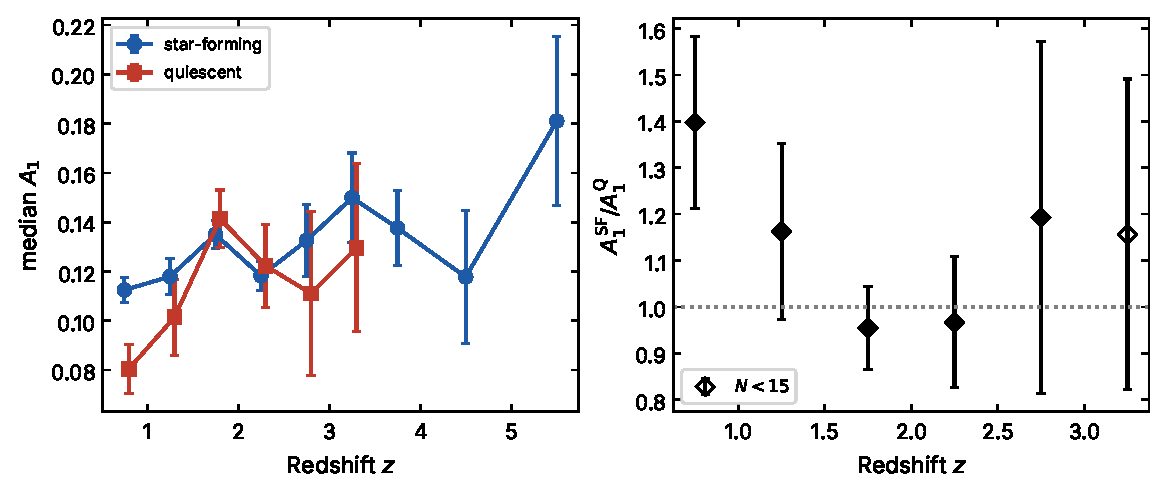
\includegraphics[width=0.95\textwidth]{Fig7_sfr.pdf}
\caption{\textit{Left:} median corrected $A_1$ of star-forming and
quiescent disks with aperture S/N$>100$. \textit{Right:} their ratio;
open symbols mark bins with fewer than 15 galaxies in a class. The two
classes have equal $A_1$ within the uncertainty at $z\lesssim3$,
$A_1^{\rm SF}/A_1^{\rm Q}=\numSFQ\pm\numSFQerr$, so in this
high-S/N subsample $A_1$ does not depend detectably on whether a disk is
forming stars. Above $z\sim3$ the quiescent sample at S/N$>100$ becomes
too small for the test.}
\label{fig:sfr}
\end{figure*}

\subsection{Early-type galaxies}\label{sec:early}

Early-type ($n>3$) galaxies show the same growth of both modes, by factors of
$\numETgrowthOne$ ($A_1$) and $\numETgrowthTwo$ ($A_2$) with the noise floor
subtracted, at a lower ratio, $A_1/A_2\approx\numETratio$, at all redshifts
(Figs.~\ref{fig:amplitudes} and \ref{fig:ratio}). That both modes also grow in a
population that is not disk-supported suggests that the growth is not peculiar
to thin disks. Because these galaxies are not thin disks, however, their
deprojected $A_2$ and the ratio correction derived from disk simulations are only
approximate, and the comparison is qualitative.

%% -----------------------------------------------------------------------
\section{Discussion}\label{sec:discussion}

\subsection{Interpretation}\label{sec:interpretation}

Our central result is that the $m=1$ and $m=2$ amplitudes of face-on,
low-S\'ersic-index galaxies grow together, by factors of $\numAOneGrowth\pm0.3$
and $\numATwoGrowth\pm0.3$ between $z\sim0.75$ and $z>4$ and with equal
logarithmic slopes, in a sample limited to the S/N range in which the calibration
gives the same answer in deep and shallow fields. They do so also at fixed
rest-frame wavelength, while their ratio stays at $\approx\numRatioMean$ or falls
slightly. The growth is smaller than the factors of 2.0 and 2.3 that the sample
without an S/N limit gives. For $A_2$ it is found at every annulus radius we
tested (factors of 1.5--1.7). In the subsamples its factor ranges from 1.3 to
2.6 and exceeds unity in all of them, but with low significance in the smallest
ones (1.3 and 1.4 in the two mass slices above $\log\Mstar=9.5$,
$1.44\pm0.47$ in the middle S/N tercile; Tables~\ref{tab:robust} and
\ref{tab:selection}). For $A_1$ it is specific to the
$0.5$--$1.5\,r_d$ annulus: it is 1.2 in an annulus 0.6 times smaller and 2.6 in
one 1.68 times larger, and it is not established at fixed resolution
(Sect.~\ref{sec:caveats}). The two modes therefore grow together in the adopted
annulus and the S/N-limited sample, and the evidence is firmer for $A_2$ than
for $A_1$. The larger $A_2$ growth is, however, the more sensitive to a single
field: PRIMER-UDS raises it, and without the two UDS mosaics the growth factors
are $1.48\pm0.20$ ($A_1$) and $1.57\pm0.18$ ($A_2$; Sect.~\ref{sec:closure}).
In the high-S/N subsample at $z\lesssim3$
the amplitudes do not differ between star-forming and quiescent disks.

This coherent evolution bears differently on each of the mechanisms outlined
in Sect.~\ref{sec:intro}. If internal lopsided modes of cold disks
\citep{Jog1997,Saha2007,2011Ap.....54..184M,2025A&AT...35..215O,2024AstBu..79..221M} or one-sided accretion
\citep{Bournaud2005,Dekel2009} dominated, $A_1$ would grow on its own and the
ratio would rise with redshift; it does not. Bar formation
\citep{Athanassoula2003,Debattista2000} would raise $A_2$ alone and lower the
ratio; this is not observed either. The parallel growth of both modes suggests
instead that the rest-frame near-infrared light of high-redshift galaxies is less
axisymmetric overall, as expected when several low-order harmonics are driven by
the same irregular, non-equilibrium light distribution. Clumpy, patchy in-situ
star formation, ongoing cold accretion and interactions can each add power to
several $m$ at once. Visual studies of these samples indeed show clumpy,
irregular rest-frame near-infrared morphologies
\citep{Ferreira2022,Kartaltepe2023}, as do the giant clumps of $z\sim2$ disks
seen in rest-frame optical and H$\alpha$ light \citep{Elmegreen2007,Genzel2011}.

Because the amplitudes trace light rather than mass, they cannot identify a
dynamical mechanism, and on their own they imply neither stronger bars nor a
particular origin of lopsidedness. Mass maps from spatially resolved
spectral-energy-distribution fits \citep{Jacobs2023,Nelson2024} would allow a
direct comparison with dynamical predictions; we leave this to a dedicated study.
Since $A_2$ at high redshift includes clumps and irregular structure as well as
bars, its increase does not contradict the declining bar fraction found by visual
and ellipse-fitting studies \citep{Guo2025,LeConte2024}. Those studies pick out
coherent, elongated, rotation-aligned bars from the full set of $m=2$ perturbers,
so a rise in generic $m=2$ power is compatible with a decline in this specific
morphological class. Early-type galaxies share the growth but keep a lower
ratio; because their ratio correction is approximate and their
deprojection-parameter errors have not been calibrated, we do not interpret this
difference physically.

\subsection{Comparison with previous work}\label{sec:previouswork}

\citet{LeBail2024} found large lopsided fractions in massive dusty
star-forming galaxies at $z=1.5$--3, and TNG50 predicts similar fractions at
$z\sim1.5$--2 \citep{Jimenez2025}. Our $A_1\approx{}$\numAOneMidRange\ at these
redshifts is consistent with a substantial lopsided population, and with
simulations in which cold accretion sustains $m=1$ asymmetries over several
galactic rotations \citep{Dekel2009,Dekel2020}. \citet{Ganapathy2024} did not
report a clear $A_1$--$z$ trend among 271 CEERS galaxies at $z=1$--4, whereas our
corrected $A_1$ increases by $\approx\numAOneIncr$ per cent between $z\sim1.25$
and $z\sim3.75$. Their Fourier--Laguerre amplitudes are measured at different
radii and with a different centring, so a direct comparison would require
applying both estimators to the same images. Comparisons with local measurements
likewise require matched radii, normalisation and resolution; we defer them to a
study of artificially redshifted local galaxies \citep[e.g.][]{Barden2008} that
mimics the \JWST\ pixel grid, PSF and noise correlation.

\subsection{Caveats}\label{sec:caveats}

The robustness tests of Appendix~\ref{app:robust} (Table~\ref{tab:robust})
qualify these results in several ways.

(i) Calibrating with clumpy models (four or eight Gaussian clumps carrying 20
or 30 per cent of the flux) instead of smooth S\'ersic disks gives growth factors
of \numClumpOne\ ($A_1$) and \numClumpTwo\ ($A_2$). This tests how sensitive the
calibration is to clumpy structure of the kind seen at high redshift
\citep{Ferreira2022,Kartaltepe2023}, but it does not reproduce the full range of
clump numbers, sizes and luminosities in real galaxies, so the correction factors
remain idealised. A galaxy-to-galaxy scatter of 0.15 or 0.30\,dex in the
amplitudes changes the recovered medians by at most \numSpreadMax\ per cent on
average, and repeating the self-consistent calibration changes no value by more
than $\numScShift\sigma$; the recovery correction is therefore not sensitive to
the amplitude at which it is anchored.

(ii) The amplitudes depend on the radius at which they are measured. In annuli
0.6 and 1.68 times smaller and larger than ours (i.e.\ scale-length or larger
half-light-radius conventions), $A_1$ grows by factors of \numAnnSmallOne\ and
\numAnnLargeOne\ and $A_2$ by \numAnnSmallTwo\ and \numAnnLargeTwo, and the mean
corrected ratio is \numAnnSmallR\ and \numAnnLargeR. Both modes grow at every
radius we tested, so the qualitative result is robust, but the growth factors and
the exact value of $A_1/A_2$ belong to the $0.5$--$1.5\,r_d$ annulus and should
not be extrapolated to other radii without the same calibration.

(iii) The stellar-mass distribution changes with redshift. Re-weighting the
sample to the same mass distribution in every bin gives growth factors of
\numMassOne\ ($A_1$) and \numMassTwo\ ($A_2$). A joint fit
$\log A=a+b\log(1+z)+c(\log\Mstar-10)$ to cells in redshift and mass gives
$b=\numRegBmOne\pm\numRegBmErrOne$ ($A_1$) and $\numRegBmTwo\pm\numRegBmErrTwo$
($A_2$), compared with $\numRegBOne$ and $\numRegBTwo$ without the mass term, so
the growth with redshift is not driven by the shifting mass distribution. In
fixed mass slices, however, the high-redshift bins contain few galaxies
(Table~\ref{tab:robust}), and the growth is not constrained above
$\log\Mstar=10$. For the mass-selected subsets we use the noise floor and
recovered fraction of the parent bin, because the subsets are too small for a
dedicated injection--recovery calibration; this is accurate only insofar as their
size and S/N distributions resemble those of the parent bin. The growth of both
modes is thus seen for $\log\Mstar<10$ (factors of 1.8--2.0 for $A_1$ and
1.3--1.9 for $A_2$, from 37 and 53 galaxies at $z>4$). Above this mass the
high-redshift bins are too small to test it: the 20 galaxies with
$10<\log\Mstar<10.5$ at $z>4$ give factors of 0.9 and 1.4.

(iv) Requiring galaxies to be resolved at $0.5\,r_d$ and detected at an aperture
S/N of at least 40 removes an increasing fraction of galaxies at high redshift
(Sects.~\ref{sec:data} and \ref{sec:closure}). Our results apply to this resolved,
high-S/N population, \numNvalid\ of the 6{,}597 face-on galaxies with cutouts, and
should not be extended uncritically to compact or faint high-$z$ systems: at
$z>4$ the sample retains 148 of the 402 face-on galaxies. Within the population,
the decrease of $r_d/{\rm FWHM}$ with redshift may contribute to the growth of
$A_1$. In a common window $1.3<r_d/{\rm FWHM}<2.15$, calibrated with its own
simulations, $A_2$ grows by a factor of $2.6\pm0.5$ but $A_1$ by only
$1.37\pm0.25$ (7 per cent of the bootstrap resamples give a factor $\leq1$),
compared with $1.71\pm0.19$ and $1.69\pm0.22$ for the full sample of the same run
(Table~\ref{tab:selection}). The growth of $A_1$ is therefore not established at
fixed resolution.

(v) The PSF correction of the ratio is approximate for early-type galaxies,
whose light profiles are not well matched by the thin-disk models of the
simulations. Photometric-redshift errors scatter galaxies between
neighbouring bins. Drawing each redshift from its catalogue uncertainty in 500
Monte Carlo realisations lowers the growth factors to $1.59\pm0.11$ ($A_1$) and
$1.67\pm0.06$ ($A_2$), from 1.74 and 1.71 for the same binning, and adding a
5 per cent fraction of catastrophic outliers lowers them to $1.42\pm0.08$ and
$1.54\pm0.09$. The mean corrected ratio changes by at most 0.02
(Table~\ref{tab:selection}). Among the 993 face-on galaxies with a spectroscopic
redshift, 4.0 per cent have $|\Delta z|/(1+z)>0.15$ (6 of the 27 at $z>3.5$), so
an outlier fraction of this size is realistic, although real outliers are not
spread uniformly in redshift as in the test.

(vi) The DJA catalogue gives no uncertainties for the S\'ersic axis ratio and
position angle. Deprojection errors of the size of the noise-induced ones change
the growth factors by at most 0.11. If the whole of the empirical difference
between the two position-angle estimates were a catalogue error, the growth
factor of $A_2$ would fall from 1.76 to 1.44--1.51 and the corrected $A_1/A_2$
would rise by up to 0.12 (Sect.~\ref{sec:injection}, Table~\ref{tab:calsys}), so
the absolute value of the ratio is uncertain at this level. Much larger errors
($\sigma_q=0.10$, $\sigma_{\rm PA}=10^\circ$ at all redshifts) would increase the
growth of $A_2$.

(vii) The amplitudes depend on S/N. Without an S/N limit the calibration fails
the closure test across field depth and the growth factors are inflated
(Sect.~\ref{sec:closure}); the limit of 40 is the lowest at which the test is
passed; the excess is intrinsic to the low-S/N galaxies rather than a
noise-floor, field or crowding systematic (Sect.~\ref{sec:closure}), and a single
calibration cannot remove an S/N-dependent effect, so we restrict the sample. Within the S/N-limited sample the bin-level calibration, which
applies one floor and one recovered fraction to galaxies of different S/N,
recovers the injected amplitudes to within 9 per cent in every S/N tercile of
every bin, and applying tercile-specific floors, recovered fractions and ratio
biases galaxy by galaxy changes the growth factors only from 1.62 to 1.59 ($A_1$)
and from 1.70 to 1.64 ($A_2$; uncertainties $\pm0.18$ and $\pm0.21$) and the mean
ratios by less than 0.01 (Table~\ref{tab:selection}). In the three S/N terciles
$A_1$ grows by factors of $2.0\pm0.3$, $1.5\pm0.2$ and $1.5\pm0.2$ and $A_2$ by
$1.8\pm0.4$, $1.4\pm0.5$ and $1.7\pm0.3$, from the lowest to the highest. A
residual dependence on S/N remains in one bin: at $z\sim4.5$ the lowest tercile
(median S/N of 52, 31 galaxies) has $A_1=0.29\pm0.03$, against $0.12\pm0.02$ and
$0.17\pm0.03$ in the other two, whereas at $z\sim5.5$ the terciles agree. Raising
the limit to S/N$\,\geq118$ (the median of the $z\sim5.5$ bin) gives growth
factors of $1.56\pm0.22$ and $1.57\pm0.36$. Combining this limit with the
resolution window of (iv) leaves 410 galaxies at $z\sim0.75$ and 41 at $z>4$, of
which only the 26 at $z\sim4.5$ form a bin of at least 20; there $A_1$ grows by
$1.19\pm0.24$ (16 per cent of the bootstrap resamples give a factor $\leq1$) and
$A_2$ by $1.8\pm0.4$ (3.5 per cent). The median stellar mass of this subsample
rises from $\log\Mstar=9.6$ to 9.8, and the amplitudes decrease only weakly with
mass at fixed redshift ($c=\numRegCOne\pm\numRegCErrOne$ and
$\numRegCTwo\pm\numRegCErrTwo$ per dex in the fit of (iii)), so mass does not
account for the weaker growth of $A_1$. Each of these subsamples on its own
gives only moderate evidence for growth; the evidence for $A_2$ is consistent
across them, while that for $A_1$ weakens whenever the resolution is fixed.

%% -----------------------------------------------------------------------
\section{Summary}\label{sec:summary}

\begin{enumerate}

\item Pixel-grid centring, a field-dependent astrometric offset, missing
deprojection and unmasked neighbours bias the Fourier amplitudes of high-redshift
galaxies by tens of per cent and can create a spurious plateau in $A_1/A_2$. We
correct for these effects and calibrate the noise and PSF suppression with
injection--recovery simulations based on empirical PSFs, measured noise
correlations and the S/N of each galaxy
(Figs.~\ref{fig:steps}--\ref{fig:injection}).

\item Fields of different depth provide a test of this calibration that is
independent of the simulations. It fails for galaxies with an aperture S/N below
about 40: at $z>4$ and fixed stellar mass the shallow fields give corrected
amplitudes two to three times larger than the deep ones, and the growth factors
of the sample without an S/N limit (2.0 and 2.3) are inflated by these galaxies.
Above S/N$\,=40$ the seven fields agree (Table~\ref{tab:closure}), and all our
results refer to this S/N-limited sample.

\item In the population resolved at $0.5\,r_d$ and above this S/N, $A_1$ and
$A_2$ of face-on disks grow by factors $\numAOneGrowth\pm0.3$ and
$\numATwoGrowth\pm0.3$ from $z\sim0.75$ to $z>4$, with slopes
${\rm d}\log A/{\rm d}\log(1+z)=0.38\pm0.08$ and $0.43\pm0.07$
(Fig.~\ref{fig:amplitudes}). The growth is stable under changes of the PSF model,
under resampling of the injection calibration and under an S/N-stratified
calibration (changes $\leq0.06$; Tables~\ref{tab:calsys}, \ref{tab:seeds} and
\ref{tab:selection}). Photometric-redshift scatter lowers the growth factors by
0.04--0.15, and position-angle errors of the largest size allowed by the data
would lower that of $A_2$ to about 1.5. At fixed resolution $A_2$ still grows
($2.6\pm0.5$) but the growth of $A_1$ is not significant ($1.37\pm0.25$), and in
the small subsample matched in both resolution and S/N neither is established
firmly (Table~\ref{tab:selection}). The growth persists at fixed rest-frame
wavelength (Fig.~\ref{fig:restframe}), and at $z\lesssim3$ high-S/N star-forming
and quiescent disks do not differ in $A_1$ (Fig.~\ref{fig:sfr}).

\item In the $0.5$--$1.5\,r_d$ annulus the corrected $A_1/A_2$ does not rise.
It is $\numRatioLo\pm\numRatioLoErr$ at $z<3.5$ and
$\numRatioHi\pm\numRatioHiErr$ at $z>3.5$, with a systematic uncertainty of up to
$+0.12$ from position-angle errors, and its redshift trend depends on the radius
of the annulus. Early-type galaxies show the same growth of both modes at
$A_1/A_2\approx\numETratioR$ (Fig.~\ref{fig:ratio}).

\item The growth also persists at fixed stellar mass for $\log\Mstar<10$ and
with clumpy calibration models. It depends on the radius: in an annulus 0.6
times smaller $A_1$ grows by only \numAnnSmallOne\ and in one 1.68 times larger
by \numAnnLargeOne, while $A_2$ grows by \numAnnSmallTwo\ and \numAnnLargeTwo. At fixed rest-frame
wavelength both modes grow by factors of $\approx\numRFgrowthOne$--$\numRFgrowthTwo$.
Because the amplitudes trace light rather than mass, the coherent growth of the
two modes does not by itself point to a dynamical mechanism; it is consistent
with irregular, non-equilibrium light distributions at high redshift.

\end{enumerate}

%% -----------------------------------------------------------------------

\section*{Acknowledgements}

We thank the DJA team for the public catalogue and image release
\citep{Valentino2023}. Based on observations with the NASA/ESA/CSA
\JWST. This research is supported by the Ministry of Innovative
Development of the Republic of Uzbekistan. This research made use of
Astropy \citep{astropy2022}, NumPy, SciPy, pandas, Matplotlib and Photutils.

\section*{Data Availability}

The DJA catalogues and images are public at
\url{https://dawn-cph.github.io/dja/}. The supplementary material allows the
results to be checked at three levels: (i) from the per-bin tables,
Table~\ref{tab:main} can be recomputed with Eq.~(\ref{eq:chain}); (ii) from the
per-galaxy amplitudes and the per-galaxy results of the injection runs,
Table~\ref{tab:main}, its uncertainties and Table~\ref{tab:chain} can be
regenerated without the images; and (iii) the full code (cutout retrieval, PSF
and noise measurement, amplitude measurement, injection simulations, tables and
figures) reproduces level (ii) from the public DJA data. The calibration tests
of Table~\ref{tab:calsys} and Table~\ref{tab:seeds} are reproduced by
\texttt{run\_calib\_tests.sh}, \texttt{run\_calib\_followup.sh} and
\texttt{run\_seed\_scatter.sh}, and the selection tests of
Table~\ref{tab:selection} by \texttt{run\_selection\_tests.sh},
\texttt{run\_matched\_bootstrap.sh} and \texttt{run\_snr\_check.sh}. The
diagnostic and real-sky injection tests of Sect.~\ref{sec:closure} are reproduced
by \texttt{diagnose\_excess.py}, \texttt{real\_sky\_injection.py} and
\texttt{run\_realsky\_seeds.sh}. The complete code and the supplementary data are
provided to the referees with the submission and are hosted in the repository
\url{https://github.com/Abbos998/jwst-lopsided-bisymmetric}, which will be made
public, with a Zenodo DOI, upon acceptance.

%% -----------------------------------------------------------------------
\bibliographystyle{mnras}
\bibliography{references}

%% -----------------------------------------------------------------------
\appendix

\section{Calculation chain of the corrected amplitudes}\label{app:chain}

The corrected amplitudes of Table~\ref{tab:main} follow from the measured
medians and the injection--recovery simulations through Eq.~(\ref{eq:chain}).

Table~\ref{tab:chain} lists the terms of Eq.~(\ref{eq:chain}) for each
redshift bin. The measured medians $A_m^{\rm meas}$ come from the adopted
pipeline; at $z\sim0.75$ and $z\sim4.5$ they are the last row of
Table~\ref{tab:steps}. Floors, recovered fractions and ratio biases come from the
injection--recovery simulations (Sect.~\ref{sec:injection}). $A_1/A_2$ is the
median of the per-galaxy ratios, which is not the same as the ratio of the median
amplitudes, and it is corrected with the bias $b$ of the same statistic in the
simulations. This table, Tables~\ref{tab:main} and \ref{tab:restframe} and every
number quoted in the text are generated by \texttt{make\_tex\_from\_data.py} from
the supplementary tables; the script also checks that Table~\ref{tab:steps}
(adopted pipeline) and the F444W row of Table~\ref{tab:restframe} agree with
Table~\ref{tab:main}. \texttt{verify\_table1.py} recomputes Table~\ref{tab:main}
from this table, and \texttt{reproduce\_table1.sh} regenerates both, with their
uncertainties, from the per-galaxy measurements and injection runs.





\section{Robustness tests}\label{app:robust}

\begin{table*}
\centering
\caption{Selection tests. Growth factors and mean corrected $A_1/A_2$ are
defined as in Table~\ref{tab:robust}. Each block is a separate run and should be
compared with its own reference row. For the S/N terciles the growth factors
compare the same tercile at $z>4$ and at $z\sim0.75$. $N_{0.75}$ and $N_{z>4}$ are
the numbers of galaxies at $z\sim0.75$ and $z>4$. The numbers in parentheses are
median $\log\Mstar$: for the matched subsamples, at $z\sim0.75$ and for the pooled
$z>4$ bins; for the S/N terciles, at $z\sim0.75$ followed by the range spanned by
the medians of the $z\sim4.5$ and $z\sim5.5$ bins. Uncertainties: for the
photometric-redshift rows, the standard deviation over the 500 Monte Carlo
realisations; for the matched subsamples and the bin-level and S/N-stratified
calibrations, bootstrap standard deviations (joint over observed and injected
galaxies for the matched subsamples, over observed galaxies for the two
calibration rows); for the S/N terciles, the bootstrap errors of the bin medians
propagated to the growth factors.}
\label{tab:selection}
\small
\begin{tabular}{lccccc}
\hline
{Test} & {$N_{0.75}/N_{z>4}$} & {$A_1$ growth} & {$A_2$ growth} &
{$\langle A_1/A_2\rangle_{z<3.5}$} & {$\langle A_1/A_2\rangle_{z>3.5}$}\\
\hline
\multicolumn{6}{l}{\textit{Photometric redshifts (500 realisations; calibration of Table~\ref{tab:chain})}}\\
Adopted redshifts (reference) & 1311/148 & 1.74 & 1.71 & 0.86 & 0.72\\
Split-normal redshift errors & -- & $1.59\pm0.11$ & $1.67\pm0.06$ & 0.86 & 0.73\\
\quad + 5 per cent catastrophic outliers & -- & $1.42\pm0.08$ & $1.54\pm0.09$ & 0.86 & 0.74\\
\multicolumn{6}{l}{\textit{Resolution and S/N matching (dedicated calibration per subsample)}}\\
Full sample (reference; $\log\Mstar=9.6$, 9.6) & 1311/148 & $1.71\pm0.19$ & $1.69\pm0.22$ & $0.86\pm0.02$ & $0.73\pm0.06$\\
$1.3<r_d/{\rm FWHM}<2.15$ (9.5, 9.6) & 440/82 & $1.37\pm0.25$ & $2.63\pm0.46$ & $0.96\pm0.03$ & $0.69\pm0.07$\\
S/N$\,\geq118$ (9.7, 9.8) & 1209/71 & $1.56\pm0.22$ & $1.57\pm0.36$ & $0.92\pm0.03$ & $0.79\pm0.11$\\
Both (9.6, 9.8)$^a$ & 410/41 & $1.19\pm0.24$ & $1.79\pm0.44$ & $1.03\pm0.04$ & $0.74\pm0.15$\\
\multicolumn{6}{l}{\textit{S/N dependence of the calibration (600 injections per bin)}}\\
Bin-level calibration (reference) & 1311/148 & $1.62\pm0.17$ & $1.70\pm0.21$ & $0.87\pm0.02$ & $0.72\pm0.05$\\
S/N-stratified calibration & 1311/148 & $1.59\pm0.18$ & $1.64\pm0.21$ & $0.87\pm0.02$ & $0.72\pm0.06$\\
Lowest S/N tercile (9.3; 9.4--9.6) & 437/48 & $2.00\pm0.33$ & $1.83\pm0.42$ & -- & --\\
Middle S/N tercile (9.6; 9.6) & 437/50 & $1.52\pm0.24$ & $1.44\pm0.47$ & -- & --\\
Highest S/N tercile (10.3; 9.6--10.1) & 437/50 & $1.46\pm0.22$ & $1.72\pm0.31$ & -- & --\\
\hline
\multicolumn{6}{l}{$^a$ The $z\sim5.5$ bin has 15 galaxies and is excluded; the growth factors use the 26 galaxies at $z\sim4.5$.}\\
\hline
\end{tabular}
\end{table*}

Table~\ref{tab:robust} repeats the final measurement with alternative choices.
Each row is corrected in the same way as Table~\ref{tab:main}
(Eq.~\ref{eq:chain}); the growth factors compare the mean of the $z\sim4.5$ and
$z\sim5.5$ bins with $z\sim0.75$, and the last two columns give the mean
corrected $A_1/A_2$ below and above $z=3.5$. \textit{Self-consistent
calibration:} a further iteration that injects the amplitudes of
Table~\ref{tab:main} tests whether the correction depends on the amplitude at
which the simulations are anchored; the change is negligible. \textit{Clumpy
calibration:} recovered fractions and ratio biases from models in which Gaussian
clumps ($\sigma=0.15\,r_d$, at $0.3$--$1.8\,r_d$) are added to the perturbed
S\'ersic disks test the sensitivity to the clumpy, irregular light distributions
typical of high-redshift galaxies \citep{Ferreira2022,Kartaltepe2023}.
\textit{Annuli:} repeating the measurement and the simulations with the annulus
scaled by 0.6 and 1.68 (0.5--1.5 in units of an exponential scale length and of a
1.68 times larger radius) tests whether the growth is tied to the particular
annulus; fewer galaxies pass the 50-pixel rule in the small annulus.
\textit{Stellar mass:} re-weighting every bin to the stellar-mass distribution of
the whole sample removes any trend induced by the shifting mass function, and the
fixed mass slices show whether the growth is driven by a particular mass range
(for the mass-selected subsets the floors and recovered fractions of the whole
bin are used). The data are in the supplementary files \texttt{review7\_*.csv}
and \texttt{mass\_test*.csv}. The tests of the deprojection parameters, the PSF
model and the sampling of the injections (Sect.~\ref{sec:injection}) are
summarised in Tables~\ref{tab:calsys} and \ref{tab:seeds}, and their outputs are
in the supplementary directory \texttt{calib\_tests/}.

Table~\ref{tab:selection} collects tests of selection effects. Each block is a
separate run with its own injection sample, so its rows should be compared with
the reference row of the same block; the reference rows differ from the nominal
row of Table~\ref{tab:robust} by the sampling of the injections
(Table~\ref{tab:seeds}). \textit{Photometric redshifts:} in each of 500
realisations every galaxy receives a redshift drawn from a split normal
distribution centred on the adopted redshift $z$, with widths $z-z_{16}$ below and
$z_{84}-z$ above it, where $z_{16}$ and $z_{84}$ are the 16th and 84th
percentiles of the catalogue. The 988 galaxies with a spectroscopic redshift keep
it; the adopted redshift lies within $[z_{16},z_{84}]$ for 98 per cent of the
galaxies, and the median $\sigma_z/(1+z)$ is 0.035. The galaxies are re-binned and
each bin is corrected with its calibration from Table~\ref{tab:chain}; without
perturbation the calculation reproduces Table~\ref{tab:main} exactly. Keeping the
calibration fixed is a reasonable approximation because, for this $\sigma_z$,
galaxies move mostly to adjacent bins, whose calibration terms are similar: their
floors differ by at most 0.012 (pipeline normalisation) and their recovered
fractions by at most 0.09 (Table~\ref{tab:chain}). In the second scenario
5 per cent of the photometric redshifts are replaced by values drawn uniformly in
$0.5<z<6$; the measured outlier fraction is 4.0 per cent
(Sect.~\ref{sec:caveats}), but real outliers are not uniformly distributed, so
the scenario remains a stress test. \textit{Resolution and S/N:} the galaxies are restricted to a
common window in $r_d/{\rm FWHM}$ (the overlap of the 10th--90th percentile
ranges of all bins) and/or to a common minimum S/N (the median S/N of the
$z\sim5.5$ bin), and each subsample is calibrated with simulations drawn from
the same window. Their uncertainties come from a joint bootstrap
(1000 resamples) of the observed galaxies of each bin and of the injected
galaxies of its calibration. The S/N distributions of the low- and high-redshift bins
overlap little even above the limit of 40 (median S/N $\approx500$ at $z\sim0.75$
and $\approx100$ at $z\sim4.5$), so a common S/N window is not possible. \textit{S/N dependence of
the calibration:} 600 galaxies per bin are injected, the injected and the
observed galaxies of each bin are split into S/N terciles, and each galaxy is
corrected with the floor, recovered fraction and ratio bias of its own tercile.
Uncertainties are bootstrap errors over the observed galaxies (for the tercile
rows, propagated from the bootstrap errors of the bins); the sampling of
the injections adds about 0.05 to the growth factors. The outputs are in the
supplementary directory \texttt{selection\_tests/}.








\bsp	% typesetting comment
\label{lastpage}
\end{document}
